\chapter{Planejamento do Sistema}

{\color{red} Dar uma introdução sobre esse capítulo, pois alterei a ordem deles}

\section{Cronograma do Projeto}


{\color{red} Vamos fazer um único cronograma do semestre ou fazer um por semestre?? Caso a segunda opção Padronizar a apresentação deles. Decidiremos em reunião }


Todo bom projeto deve ter um cronograma e um planejamento de ação, baseado nisso, foi elaborado dois cronogramas: um apresentando todo o conteúdo aprendido no semestre e outro montando plano de ação para implementação do projeto.

As figuras a seguir, são cronogramas que demonstram a trajetória do desenvolvimento do projeto. Divididos por semestre, os cronogramas listam as atividades aprendidas nas UCs, com todas as partes teóricas e práticas onde o objetivo principal é implementar todo conhecimento adquirido em prol de um projeto único: A unificação de todas as UCs do curso de Sistemas para Internet.

\begin{figure}[htb]
	\caption{\label{cron-3-semestre}Cronograma de Aprendizagem: Terceiro Semestre}
	\begin{center}
		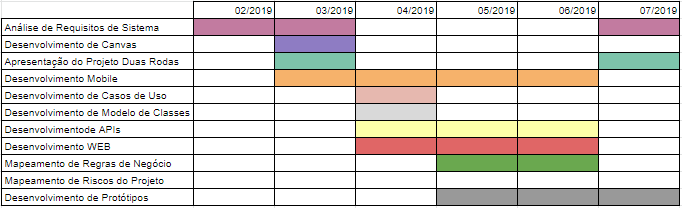
\includegraphics[scale=0.90]{./Figuras/cronograma-3-semestre.png}
	\end{center}
\end{figure}


\begin{figure}[htb]
	\caption{\label{cron-4-semestre}Cronograma de Aprendizagem: Quarto Semestre}
	\begin{center}
		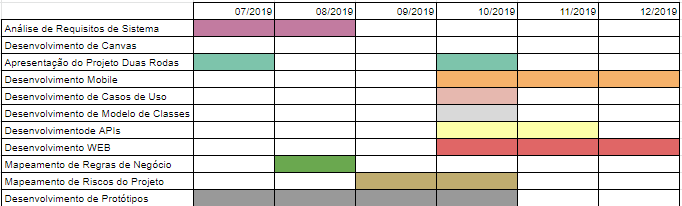
\includegraphics[scale=0.90]{./Figuras/cronograma-4-semestre.png}
	\end{center}
\end{figure}


\begin{figure}[htb]
	\caption{\label{cron-4-semestre}Cronograma de Aprendizagem: Quinto Semestre}
	\begin{center}
		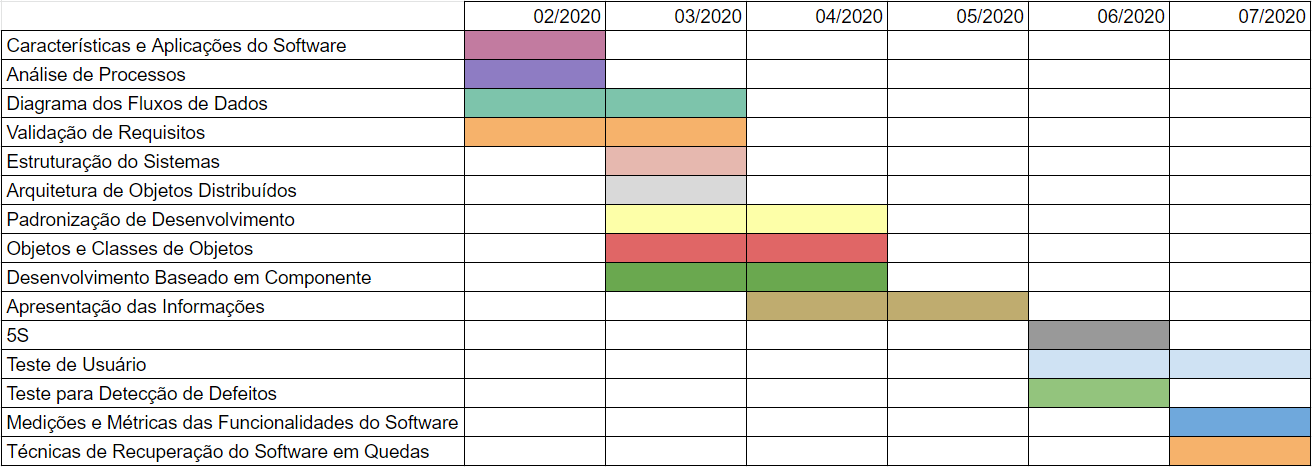
\includegraphics[scale=0.70]{./Figuras/cronograma-5-semestre.png}
	\end{center}
\end{figure}


{\section{Análise de riscos}
	
	A análise de riscos tem como objetivo identificar os possíveis problemas durante e após o desenvolvimento do projeto a fim de elaborar um plano de ação para solucionar rapidamente o problema de fato \cite{schmitzanalise}.
	
	Segundo \cite{de2003engenharia}, um grande volume de dados publicados aponta para os riscos que correm os projetos de software executados sem a utilização de processos adequados. Um levantamento publicado, a partir de
	uma base de dados de 4.000 projetos, constatou a ocorrência frequente dos seguintes
	problemas: 
	
	\begin{itemize}
		
		\item 70\% dos projetos de grandes aplicativos sofre de instabilidade dos requisitos. Os requisitos crescem tipicamente cerca de 1\% ao mês, atingindo níveis de mais de 25\% de inchaço ao final
		do projeto.
		
		\item Pelo menos 50\% dos projetos são executados com níveis de produtividade abaixo do normal.
		
		\item Pelo menos 25\% do software de prateleira e 50\% dos produtos feitos por encomenda apresentam níveis de defeitos superiores ao razoável. 
		
		\item Produtos feitos sob pressão de prazos podem quadruplicar o número de defeitos.
		
		\item Pelo menos 50\% dos grandes projetos de software estouram seu orçamento e seu prazo. 
		
	\end{itemize}
	
	
	Sendo assim, foi identificado os fatores de risco, no qual o projeto em questão possa estar exposto. Nela, faz-se uma análise do impacto e probabilidade de fatores prejudiciais ao projeto, conforme tabela \ref{tebela_risco} abaixo.
	
	\begin{table}[]
		\caption{\label{tebela_risco} Tabela de Riscos Agil.it}
		\begin{tabular}{l|l|l}
			\hline
			\rowcolor[HTML]{EFEFEF} 
			\textbf{Riscos}                     & \textbf{Probabilidade} & \textbf{Impacto} \\ \hline
			\rowcolor[HTML]{DD7346} 
			Mudança de escopo                   & 90\%                   & 2                \\ \hline
			\rowcolor[HTML]{DD7346} 
			Entrega no prazo                    & 70\%                   & 3                \\ \hline
			\rowcolor[HTML]{DD7346} 
			Integração com SAP                  & 70\%                   & 2                \\ \hline
			\rowcolor[HTML]{FFFE65} 
			Implantação na empresa              & 60\%                   & 2                \\ \hline
			\rowcolor[HTML]{FFFE65} 
			Conexão com o banco de dados        & 60\%                   & 3                \\ \hline
			\rowcolor[HTML]{FFFE65} 
			Aceitação da usabilidade do sistema & 50\%                   & 2                \\ \hline
			\rowcolor[HTML]{FFFE65} 
			Usuários inexperientes              & 40\%                   & 2                \\ \hline
			\rowcolor[HTML]{9AFF99} 
			Mudanças na tecnologia              & 20\%                   & 3                \\ \hline
			\rowcolor[HTML]{9AFF99} 
			Segurança dos dados                 & 15\%                   & 2                \\ \hline
			\rowcolor[HTML]{9AFF99} 
			Conexão com a rede                  & 10\%                   & 2                \\ \hline
			\rowcolor[HTML]{9AFF99} 
			Falta de profissionais              & 5\%                    & 3                \\ \hline
		\end{tabular}
		\caption{Fonte: os autores (2020)}
	\end{table}
	
	
	{\color{red} Melhorar essa explicação e dar uma introduzida no sentido de utilização das cores também, por mais obvia que seja}
	
	Na tabela \ref{tebela_risco} estão mapeados os principais riscos identificados para o projeto Agil.It. Nela, a probabilidade indica a chance do risco ocorrer e o impacto é uma escala de um a três (1-3) do quanto o risco pode afetar a conclusão e entrega do projeto. A seguir será abordado o diagrama de causa e efeito.
	
	{\subsection{Diagrama de Causa e Efeito}
		
		{\color{red} Descrever Diagrama de Causa e Efeito com referencias}
		
		
		\begin{figure}[htb]
			\caption{\label{causaeefeito1}Diagrama de Causa e Efeito}
			\begin{center}
				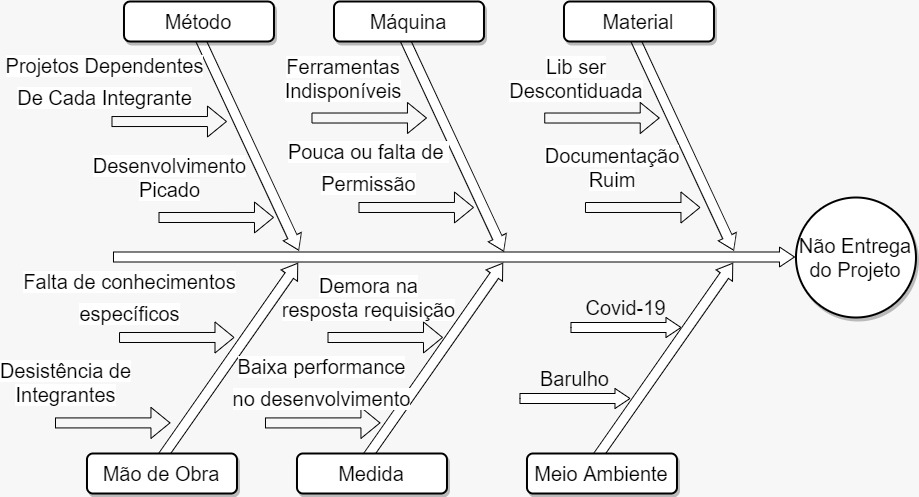
\includegraphics[scale=0.55]{./Figuras/Diagrama causa e efeito.jpeg}
			\end{center}
			\legend{Fonte: os autores (2020)}
		\end{figure}
	}
	
	
	
	\section{PMBOK}
	
	{É uma metodologia de gerenciamento de projeto internacionalmente reconhecida, essas práticas podem auxiliar na resolução dos recursos humanos, capitais, tecnológicos e técnicos. Além disso, utilizando PMBOK é possível gerir melhor o andamento do projeto e de forma mais coordenada. Segundo \cite{PMG2018} o PMBOK tem conhecimentos já comprovados que são amplamente utilizados, assim como o conhecimento de práticas mais inovadoras e avançadas} Dentre as técnicas de planejamento, pode-se utilizar para estudos e desenvolvimento a EAP -  Estrutura Analítica de Projetos, descrita a seguir.
	
	\subsection{Estrutura Analítica do Projeto}
	
	
	
	{A Estrutura Analítica do Projeto (EAP) é a divisão estruturada de trabalho do projeto dividido em faixas gerenciadas cujo a sua totalidade significa em um entregável ao projeto final.
		
		Segundo \cite{PMI2018} o detalhamento da EAP deve chegar até o nível do pacote de trabalho, nível mais baixo na EAP, que é o ponto no qual o custo e o cronograma do trabalho podem ser estimados de forma confiável. Porém o nível de detalhamento desse pacote varia de acordo com a complexidade de cada projeto. \cite{kerzner2017} defende que a EAP deve ser composta por até três níveis pois se for detalhado com demaseio o custo com o gerenciamento serão também excessivos.}
	
	Para o projeto Agil-it foi decidido utilizar 6 faixas de entregáveis:
	
	\begin{subalineas}
		\item {Planejamento};
		\item {Análise};
		\item {Implementação Web};
		\item {Implementação Mobile};
		\item {Testes};
		\item {Implantação}.
	\end{subalineas}
	
	
	\begin{landscape}
		\begin{figure}[htb]
			\caption{\label{EAP}EAP AGIL.IT}
			\begin{center}
				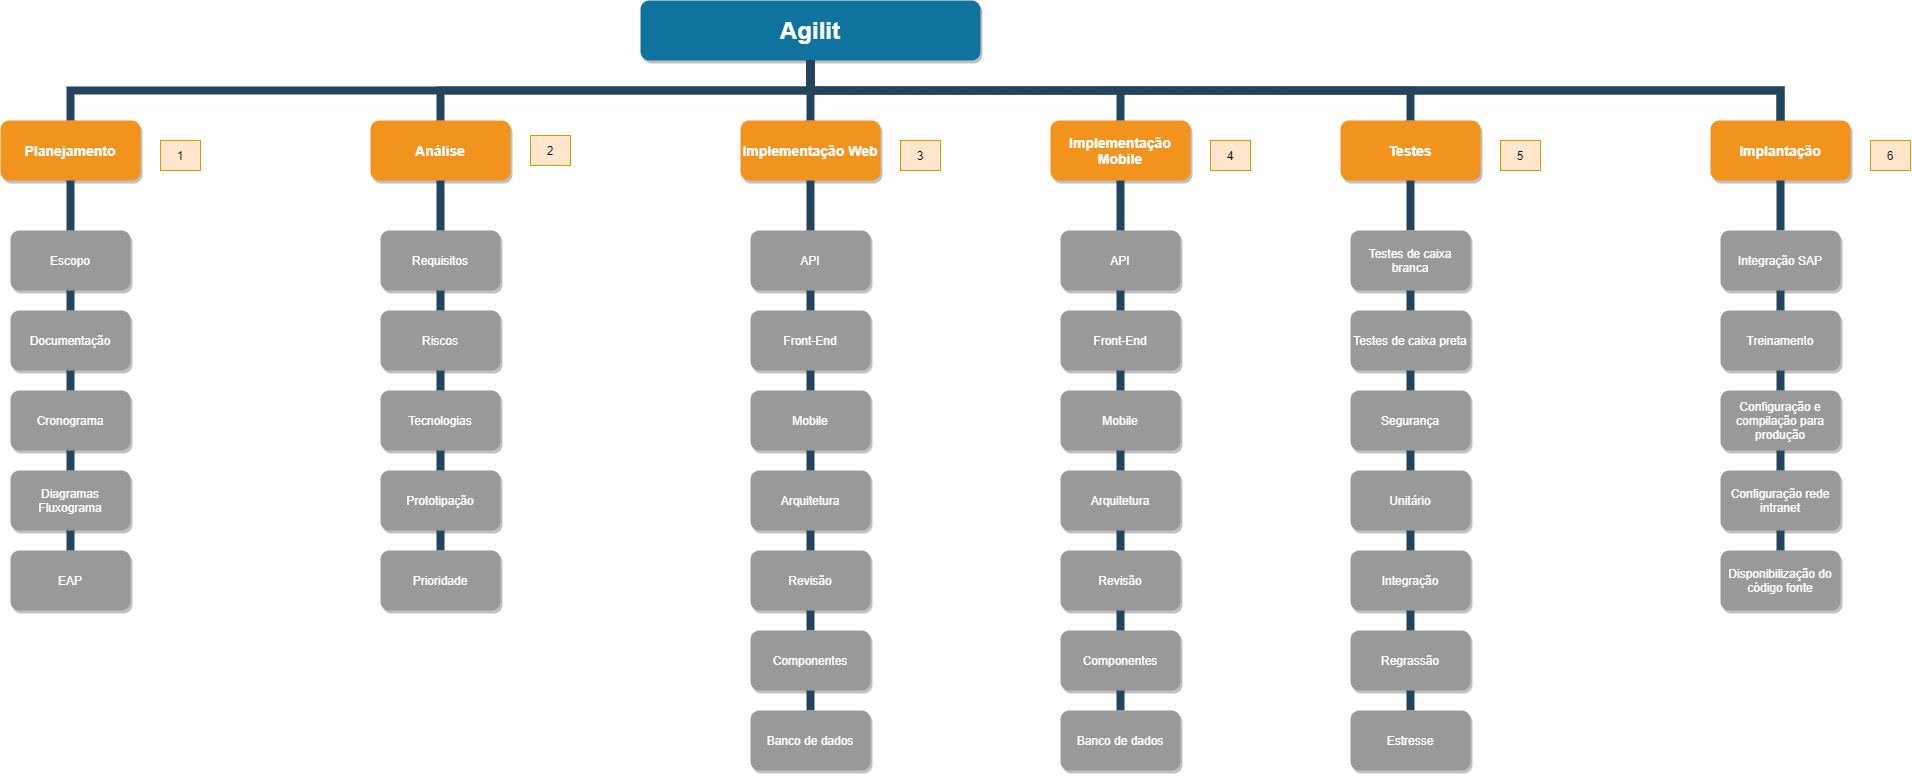
\includegraphics[scale=0.38]{./Figuras/EAP.png}
			\end{center}
			\legend{Fonte: os autores (2020)}
		\end{figure}
	\end{landscape}
	
	A figura \ref{EAP} mostra a estrutura e o desenvolvimento que cada faixa requer no projeto. Ela não segue uma ordem cronológica, portanto não é necessário finalizar uma faixa para começar outra, muitas vezes elas são desenvolvidas em conjunto para uma melhor utilização do tempo de projeto.
	
	
	\subsection{Fluxo de Processos}
	% ---
	
	{O fluxo de processo é subdividido em cinco fases principais sobre o fluxo do projeto, iniciação sendo a primeira seguindo de planejamento, execução, monitoramento, controle e finalização. Para \cite{PMG2018} um projeto é desenvolvido a partir de uma idéia, em seguida parte para um plano e após isso é executado e concluído.}
	
	Para a definição dos processos, foi utilizado os seguintes recursos:
	
	\begin{subalineas}
		\item {Partes Interessadas};
		\item {Escopo};
		\item {Tempo};
		\item {Recursos Humanos};
		\item {Aquisições};
		\item {Qualidade};
		\item {Comunicações};
		\item {Riscos}.
	\end{subalineas}
	
	A figura abaixo contém todos os fluxos desenhados para o projeto.{\color{red}chamar pelo numero da figura não abaixo}
	{\color{red} Usar h para forçar a imagem ficar no local}
	
	\begin{figure}[h]
		\caption{\label{Fluxo-Processos}Fluxo e Processos AGIL.IT}
		\begin{center}
			\includegraphics[scale=0.24]{./Figuras/fluxo-processos.png}
		\end{center}
		\legend{Fonte: os autores (2020)}
	\end{figure}
	
	
	
	{\textbf{Iniciação} - Esta é a fase inicial do projeto, nela é determinado a necessidade do projeto, com seus objetivos e justificativas, então é realizado os documentos iniciais onde as melhores estratégias são identificadas e selecionadas.}
	
	{\textbf{Planejamento} - Fase onde deve ser detalhado minuciosamente tudo aquilo que será realizado no projeto, desde cronogramas, interdependências entre atividades, alocação dos recursos envolvidos, análise de custos etc. Esta parte é muito importante pois a execução do projeto será em cima destas atividades para que sejam executadas sem dificuldades e imprevistos.}
	
	{\textbf{Execução} - Nesta fase tudo é onde tudo que foi planejado anteriormente se torne realidade, tendo que ser executado e realizado conforme planejado, qualquer erro cometidas nas fases anteriores fica evidente durante essa fase. }
	
	{\textbf{Monitoramento e Controle} - Esta fase acontece paralelamente às demais fases do projeto, acompanhando e controlando aquilo que está sendo realizado no projeto como um todo, podendo propor ações corretivas e preventivas no menor espaço de tempo possível após a detecção de erros.}
	
	
	\section{Protótipo}
	
	{\color{red} Reduzir o numero de imagens dessa section}
	
	A prototipação é uma etapa de suma importância no desenvolvimento de projeto de software. Além de melhorar a produtividade da equipe, ela facilita o entendimento dos requisitos do sistema e permite a apresentação de de conceitos e funcionalidades da aplicação de modo simplificado.
	Nesse trabalho foi utilizado a prototipação visual cujo ênfase se aplica a estética e usabilidade. Nesse tipo de protótipo é possível identificar o layout e a identidade visual da aplicação. \cite{dextra2013prototipacao}
	
	{Protótipos podem ser gerados de acordo com as seguintes categorias \cite{coyette2004sketchixml}: protótipos em baixa fidelidade que focam na interação, em componentes de interface e na estrutura geral do sistema; protótipos em alta fidelidade que produzem uma imagem real do sistema; protótipos executáveis que produzem o código em uma linguagem de programação, focando em navegação, mas sem ainda levar em consideração as regras de negócio. Cada categoria serve para um propósito específico: protótipos em baixa fidelidade são úteis para demonstrar aos usuários quais atividades o sistema atende e as possibilidades de navegação no sistema, assim como para proporcionar uma visão geral do sistema. Protótipos em alta fidelidade são úteis para demonstrar padrões e guias de estilo. Protótipos executáveis são úteis para demonstrar navegação e testar o uso da interface \cite{rosemberg2008prototipaccao}.Seguindo as definições, o projeto desenvolvido utiliza os protótipos de baixa fidelidade}
	
	\section{Aplicação WEB}
	A aplicação web tem como foco o gerenciamento de toda a aplicação envolvendo consultas e cadastros gerais do sistema.
	Apesar desse foco acentuado à gestão, é possível desempenhar todos os papeis dentro da aplicação web.
	
	
	\subsection{Login}
	
	\begin{figure}[htb]
		\caption{\label{web_login}Tela de Login do Agil.It}
		\begin{center}
			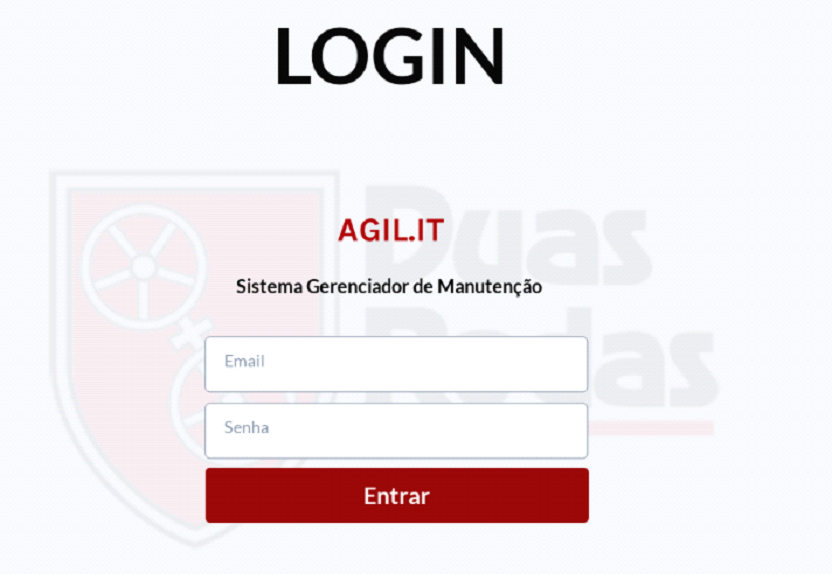
\includegraphics[scale=0.70]{./Figuras/web/login.png}
		\end{center}
		\legend{Fonte: os autores (2020)}
	\end{figure}
	
	A tela \ref{web_login} será a página responsável por autenticar os usuários e garantir a segurança do sistema.
	
	
	\subsection{Cadastro de Ordem de Manutenção}
	
	\begin{figure}[htb]
		\caption{\label{web_cad-om}Cadastro de Ordem de Manutenção}
		\begin{center}
			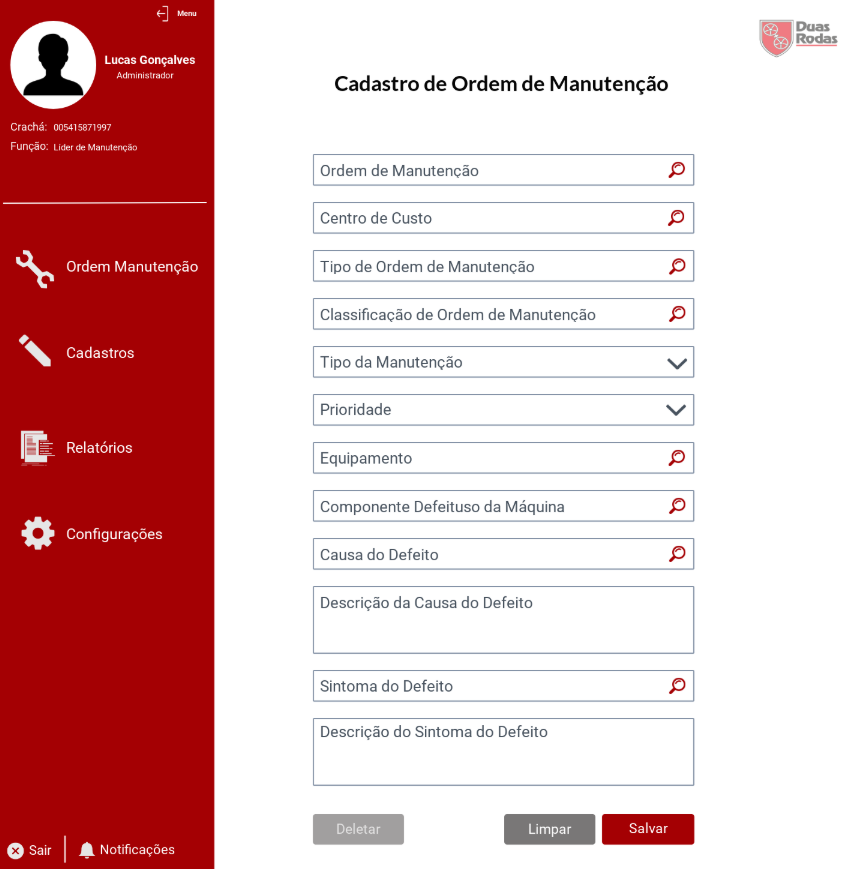
\includegraphics[scale=0.65]{./Figuras/web/cad-om.png}
		\end{center}
		\legend{Fonte: os autores (2020)}
	\end{figure}
	
	Na tela \ref{web_cad-om} é cadastrada e atualizada ordens de manutenção. Ela terá acesso às operações, componentes e assinaturas.
	
	
	\subsection{Monitor de Ordem de Manutenção: Cards}
	
	\begin{figure}[htb]
		\caption{\label{web_monitor-om-card}Monitor de Ordem de Manutenção: Cards}
		\begin{center}
			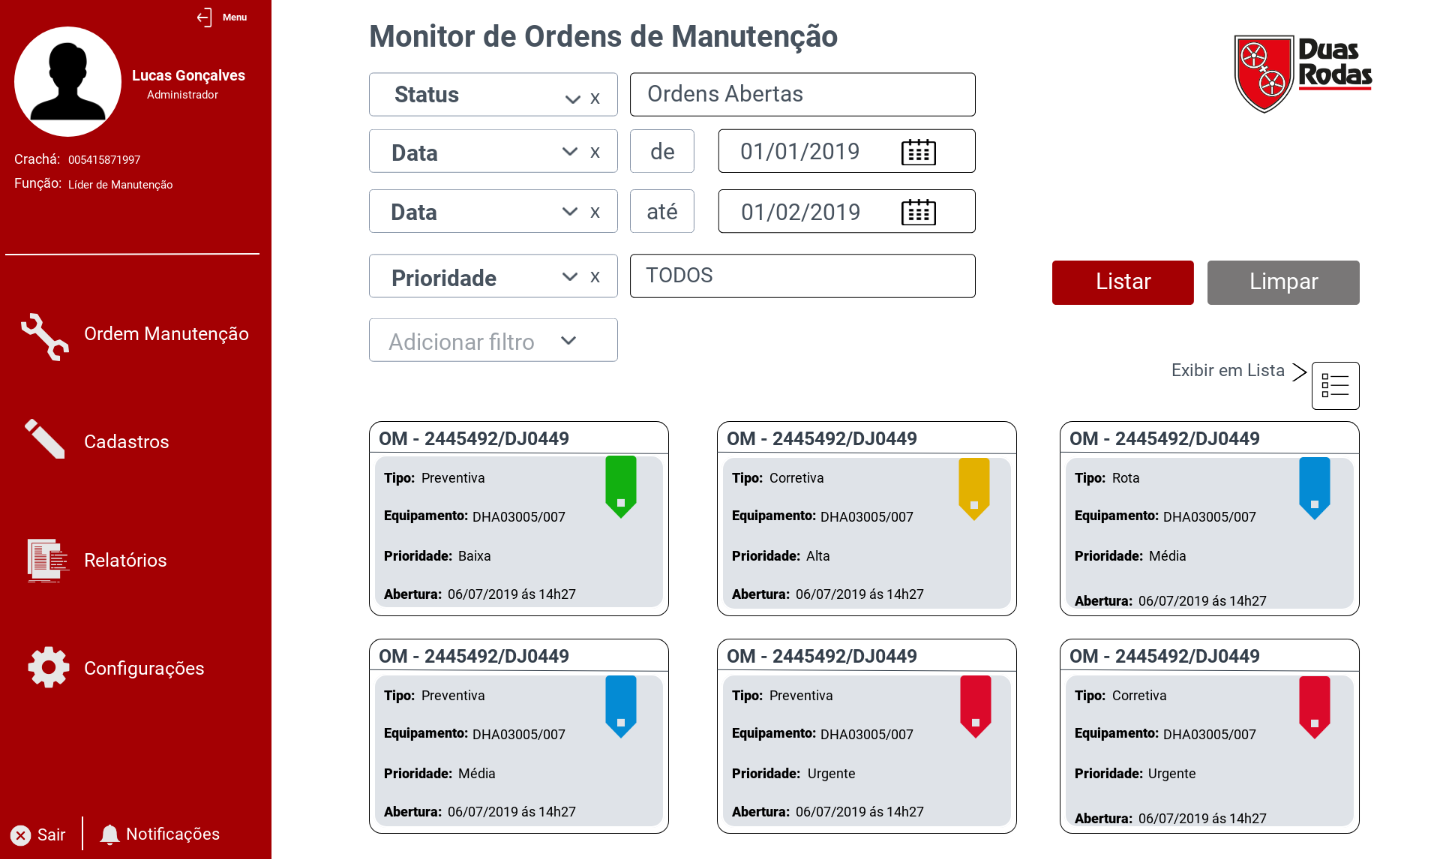
\includegraphics[scale=0.45]{./Figuras/web/monitor-om-card.png}
		\end{center}
		\legend{Fonte: os autores (2020)}
	\end{figure}
	
	A tela \ref{web_monitor-om-card} permite a consulta rápida e dinâmica das ordens de manutenção. Nela você pode aplicar os filtros de acordo com as \newline necessidades e será listada em forma de cartões, eles darão acesso à uma tela de detalhamento de ordem de manutenção.
	
	\newpage
	\subsection{Monitor de Ordem de Manutenção: Listas}
	
	\begin{figure}[htb]
		\caption{\label{web_monitor-om-lista}Monitor de Ordem de Manutenção: Listas}
		\begin{center}
			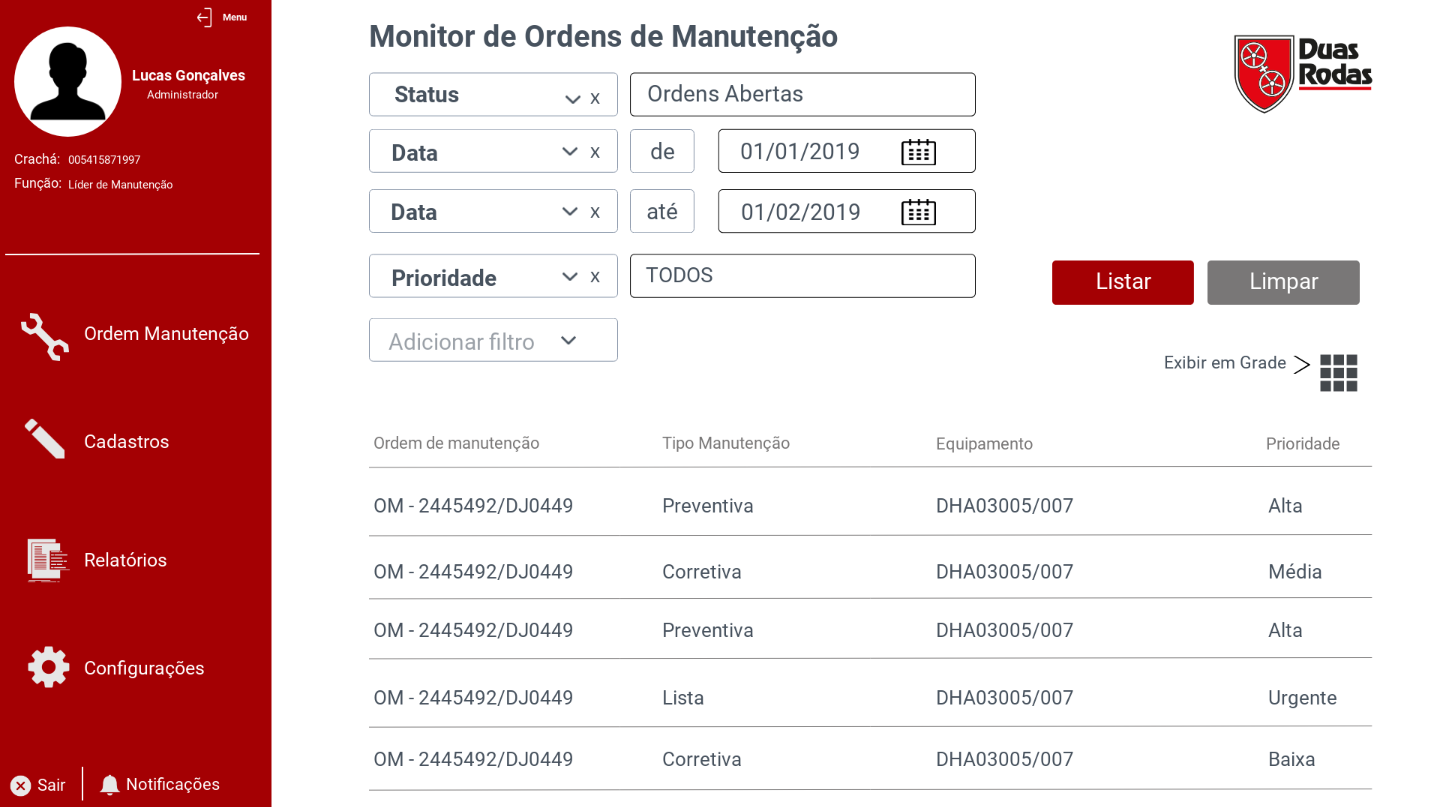
\includegraphics[scale=0.45]{./Figuras/web/monitor-om-lista.png}
		\end{center}
		\legend{Fonte: os autores (2020)}
	\end{figure}
	
	A tela \ref{web_monitor-om-lista} permite a consulta rápida e dinâmica das ordens de manutenção. Nela você pode aplicar os filtros de acordo com as \newline necessidades e será listada em forma de listas, eles darão acesso à uma tela de detalhamento de ordem de manutenção.
	
	\newpage
	\subsection{Ordem de Manutenção}
	
	\begin{figure}[htb]
		\caption{\label{web_om-capa}Ordem de Manutenção}
		\begin{center}
			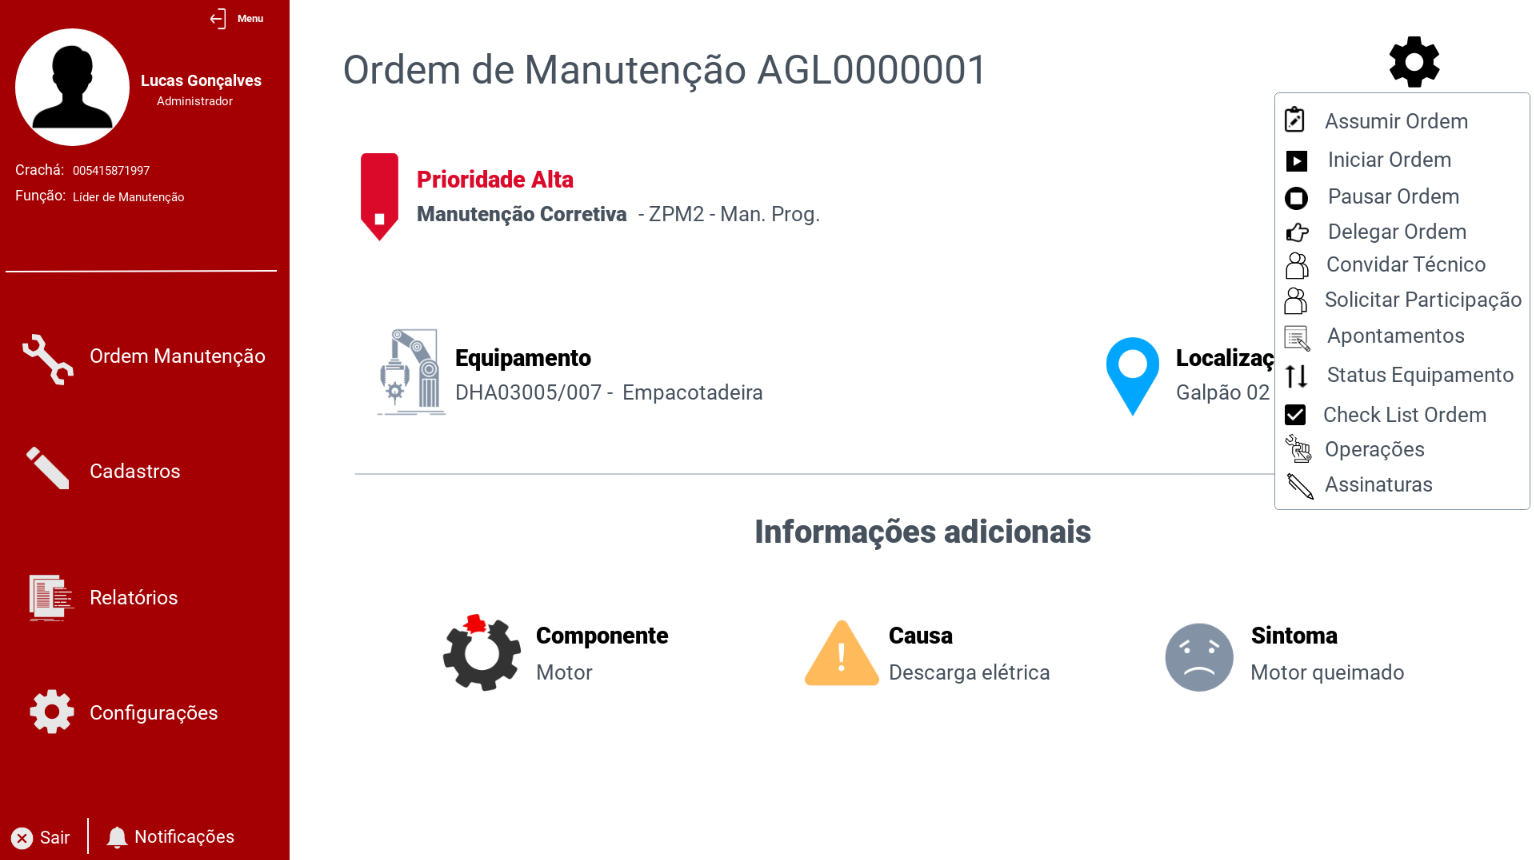
\includegraphics[scale=0.40]{./Figuras/web/om-capa.png}
		\end{center}
		\legend{Fonte: os autores (2020)}
	\end{figure}
	
	Na tela \ref{web_om-capa} será possível acompanhar o andamento de uma ordem de manutenção de lista, ver informações referente à ordem e executar ações nela, como alterar status, adicionar operações e realizar assinaturas.
	
	\newpage
	\subsection{Checklist de Segurança}
	
	\begin{figure}[htb]
		\caption{\label{web_check-list}Checklist de Segurança}
		\begin{center}
			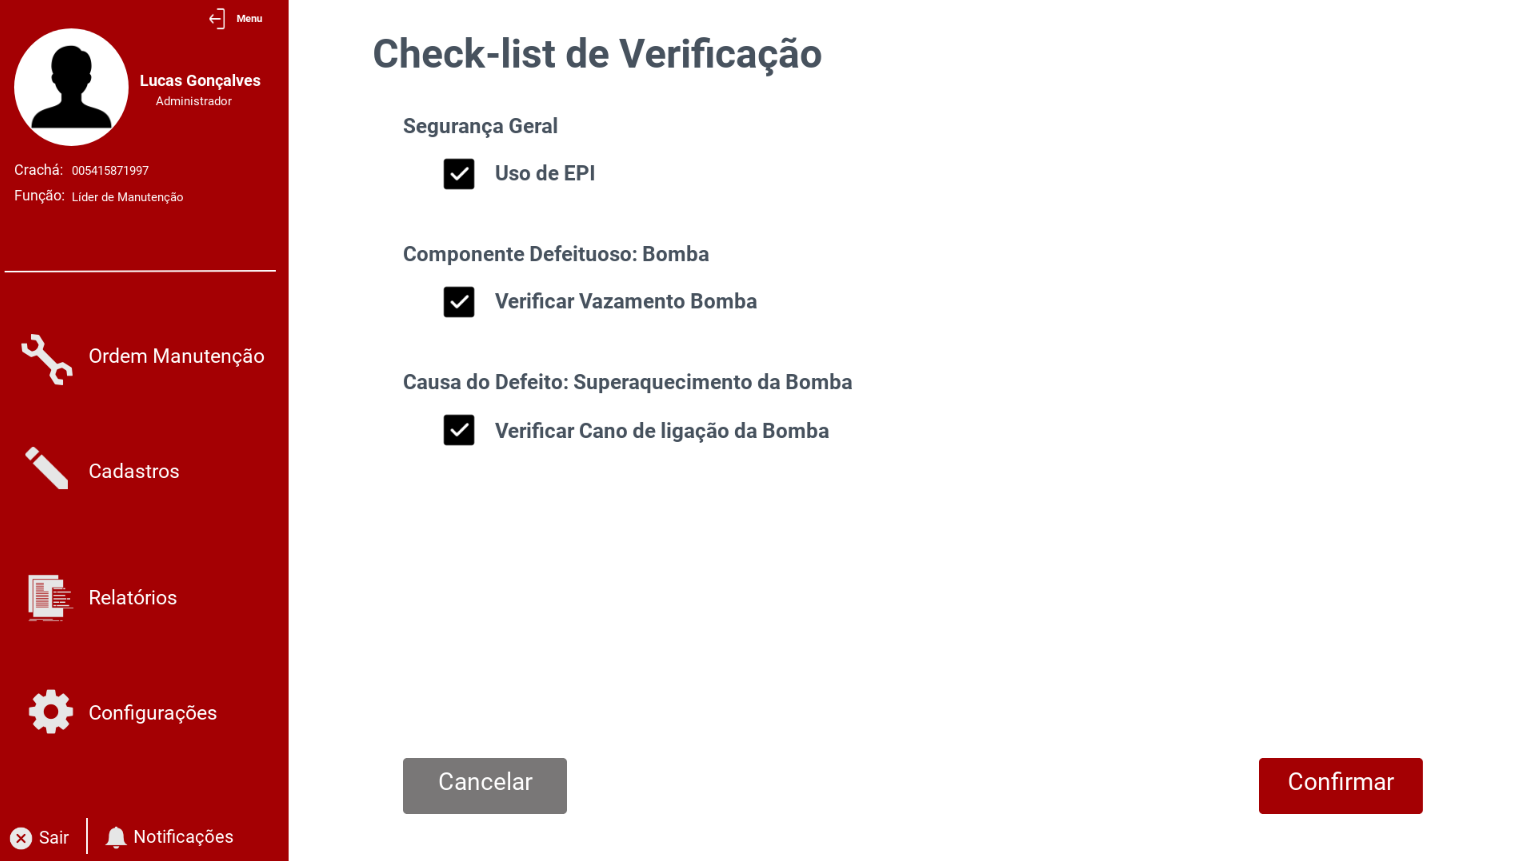
\includegraphics[scale=0.40]{./Figuras/web/check-list.png}
		\end{center}
		\legend{Fonte: os autores (2020)}
	\end{figure}
	
	Na tela \ref{web_check-list} o manutentor irá marcar a lista de segurança antes de iniciar a ordem de manutenção.
	
	\newpage
	\subsection{Operações da Ordem de Manutenção}
	
	\begin{figure}[htb]
		\caption{\label{web_om-operacoes}Operações da Ordem de Manutenção}
		\begin{center}
			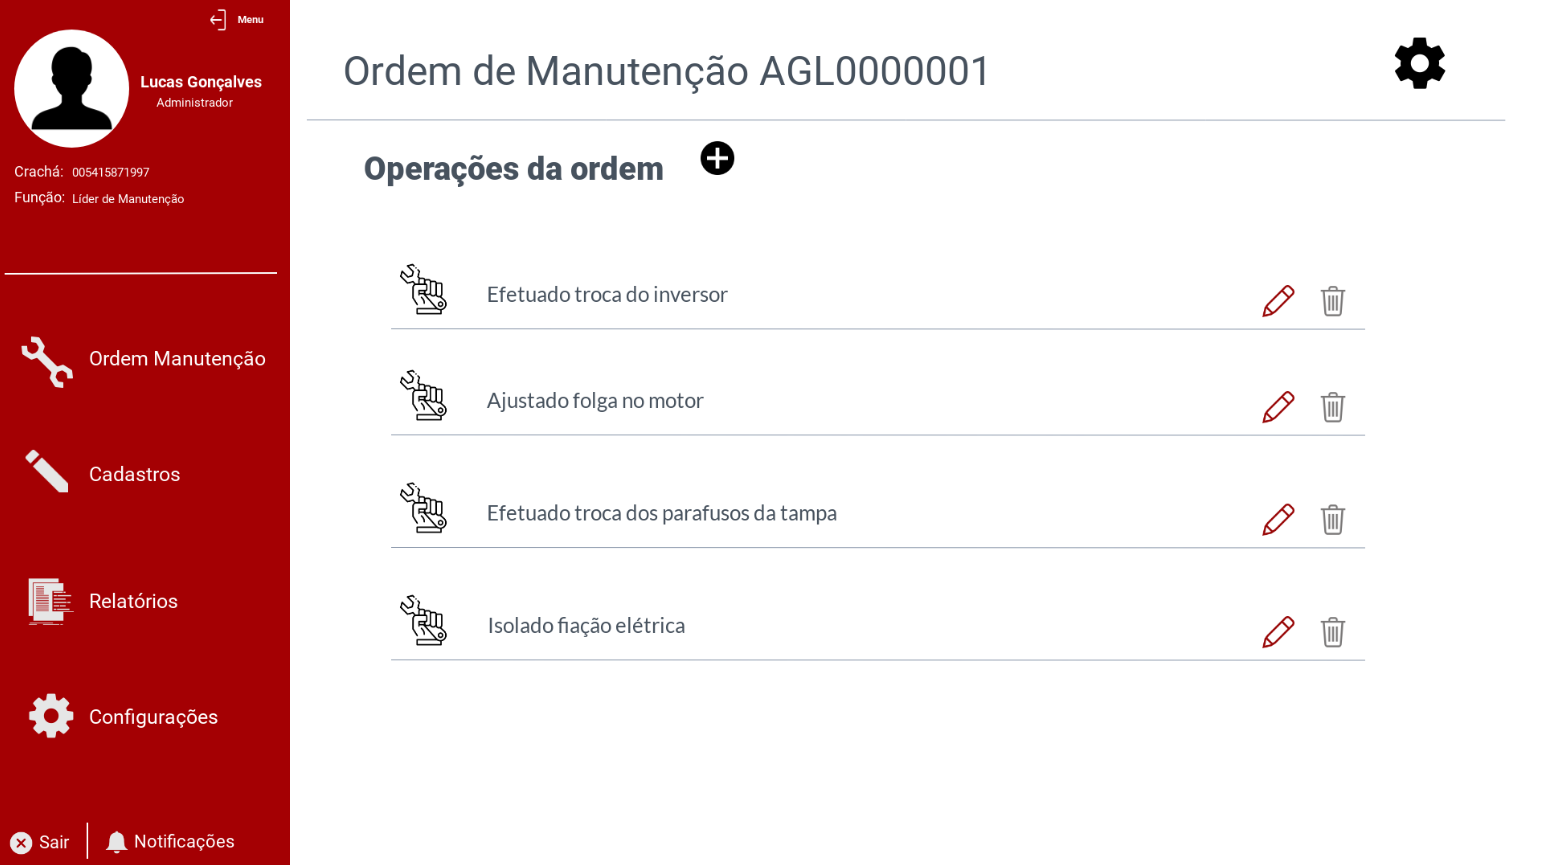
\includegraphics[scale=0.40]{./Figuras/web/om-operacoes.png}
		\end{center}
		\legend{Fonte: os autores (2020)}
	\end{figure}
	
	Na tela \ref{web_om-operacoes} é possível verificar todas as operações pré cadastradas para a OM e cadastrar novas operações conforme necessidade para o andamento da OM.
	
	\newpage
	\subsection{Ordem de Manutenção: Lista}
	
	\begin{figure}[htb]
		\caption{\label{web_om-lista}Ordem de Manutenção: Lista}
		\begin{center}
			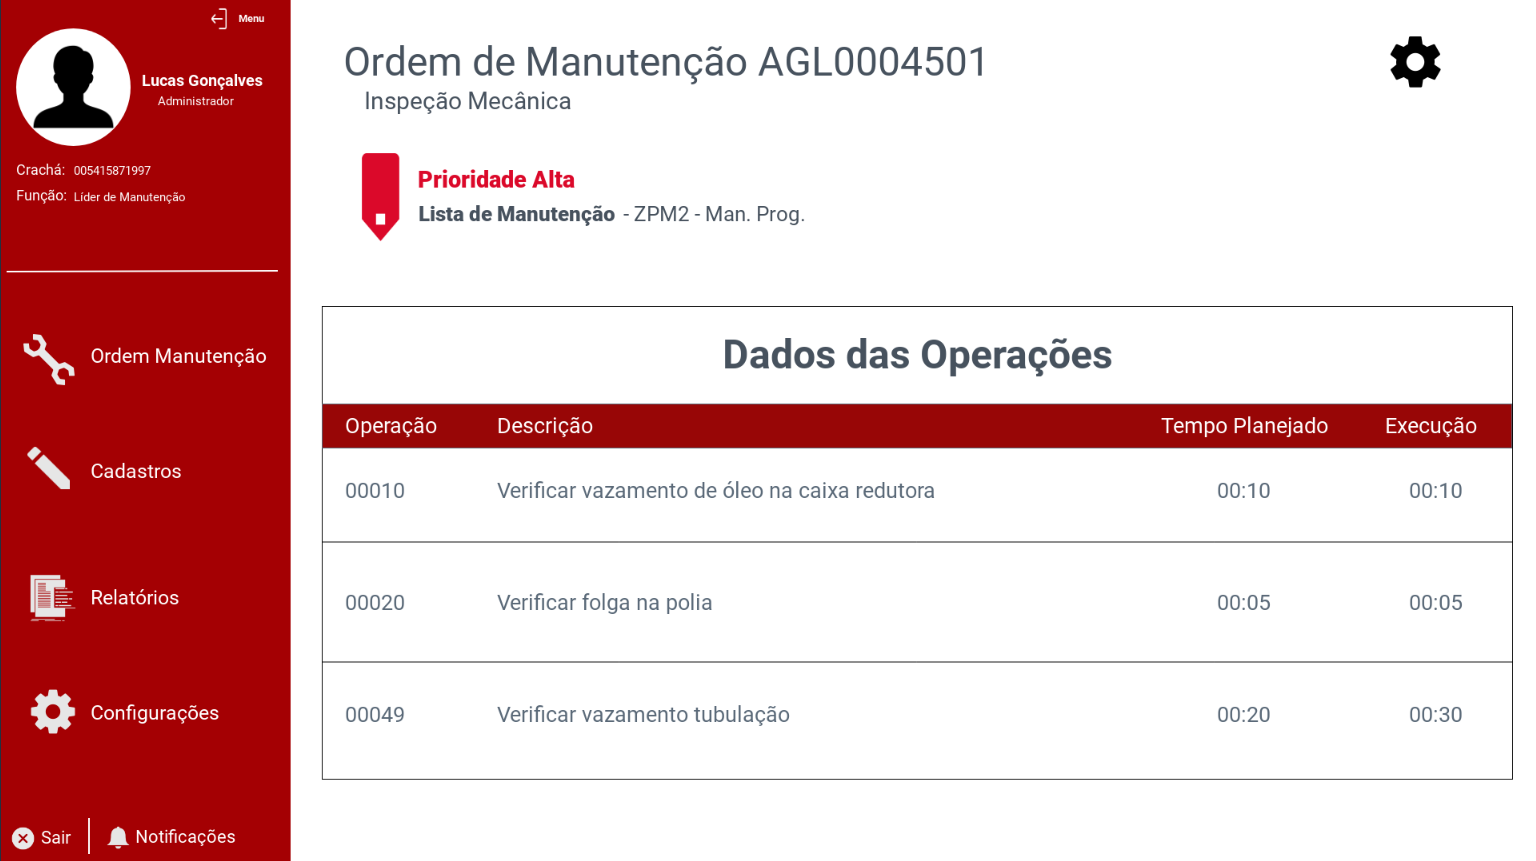
\includegraphics[scale=0.40]{./Figuras/web/om-lista.png}
		\end{center}
		\legend{Fonte: os autores (2020)}
	\end{figure}
	
	Na tela \ref{web_om-lista} será possível acompanhar o andamento de uma ordem de manutenção de lista, ver informações referente à ordem e executar ações nela, como alterar status, adicionar operações e realizar assinaturas.
	
	\newpage
	\subsection{Equipamentos da Ordem de Manutenção: Lista}
	
	\begin{figure}[htb]
		\caption{\label{web_om-lista-equipamentos}Equipamentos da Ordem de Manutenção: Lista}
		\begin{center}
			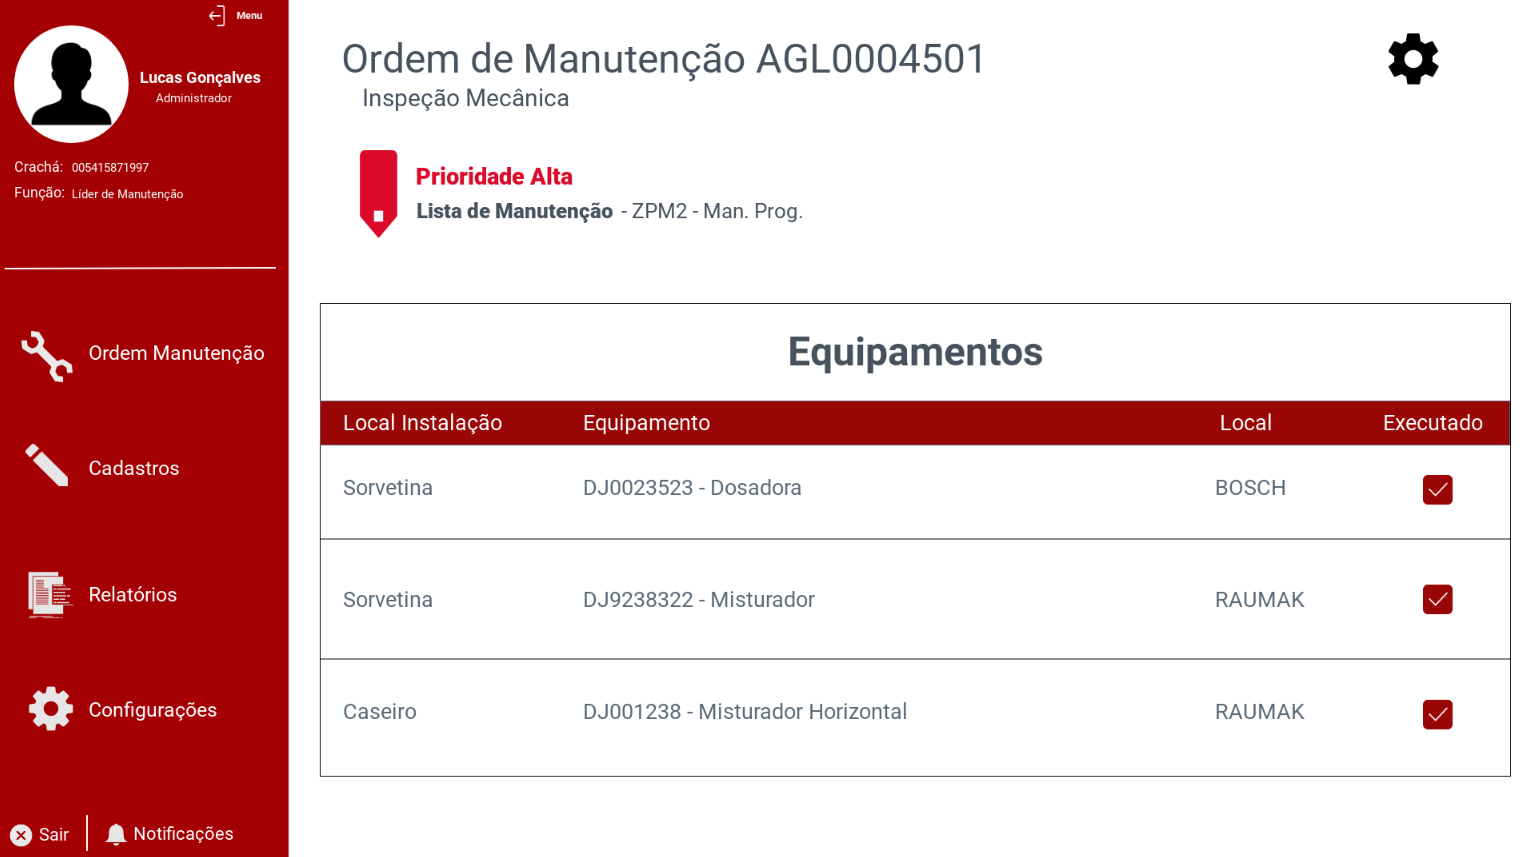
\includegraphics[scale=0.40]{./Figuras/web/om-lista-equipamentos.png}
		\end{center}
		\legend{Fonte: os autores (2020)}
	\end{figure}
	
	Na tela \ref{web_om-lista-equipamentos} será possível acompanhar os equipamentos que terão de ser inspecionados pelo manutentor e o mesmo marcar se executou ou não.
	
	\newpage
	\subsection{Ordem de Manutenção: Rota}
	
	\begin{figure}[htb]
		\caption{\label{web_om-rota}Ordem de Manutenção: Rota}
		\begin{center}
			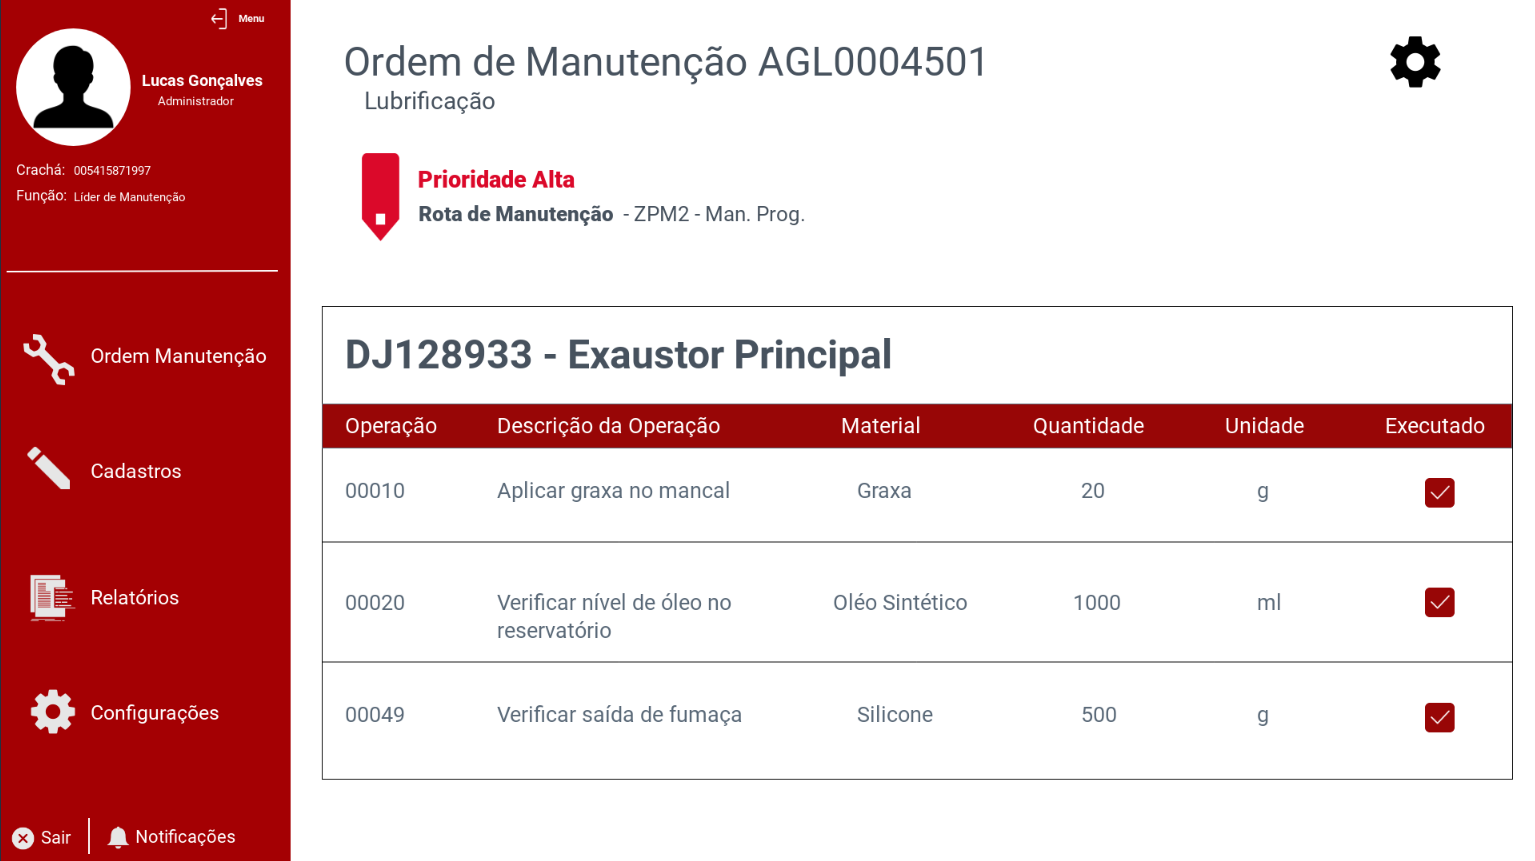
\includegraphics[scale=0.40]{./Figuras/web/om-rota.png}
		\end{center}
		\legend{Fonte: os autores (2020)}
	\end{figure}
	
	Na tela \ref{web_om-rota} será possível acompanhar o andamento de uma ordem de manutenção de lista, ver informações referente à ordem e executar ações nela, como alterar status, adicionar operações e realizar assinaturas.
	
	\newpage
	\subsection{Convidar ou Delegar Ordem de Manutenção}
	
	\begin{figure}[htb]
		\caption{\label{web_om-convidar-delegar}Convidar ou Delegar Ordem de Manutenção}
		\begin{center}
			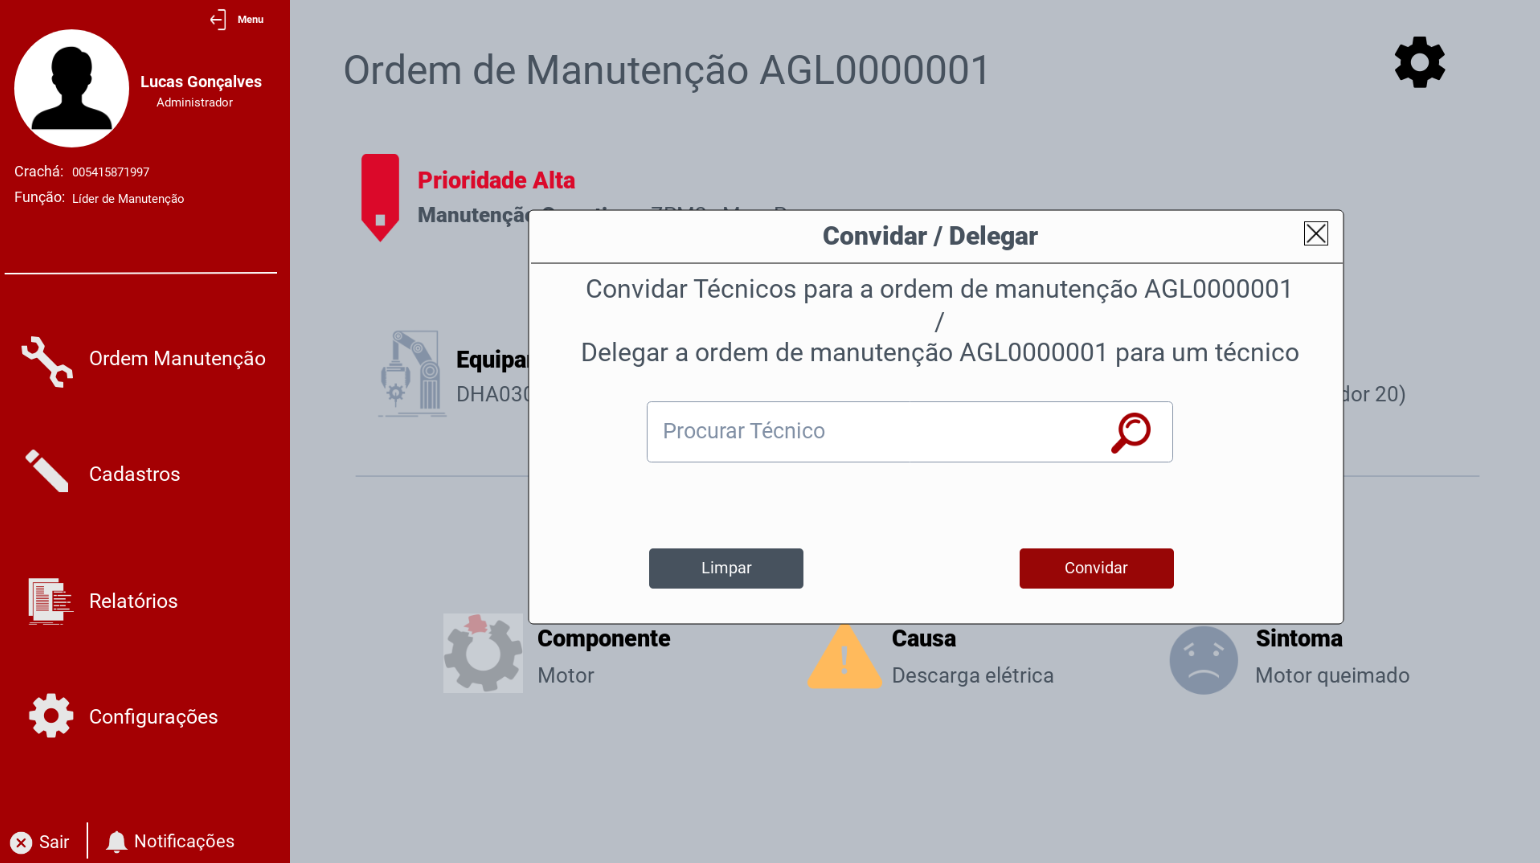
\includegraphics[scale=0.40]{./Figuras/web/om-convidar-delegar.png}
		\end{center}
		\legend{Fonte: os autores (2020)}
	\end{figure}
	
	Na tela \ref{web_om-convidar-delegar} será possível convidar técnicos para se juntarem a ordem de manutenção ou delegar a ordem de manutenção a outro manutentor. Ação só permitida àqueles que são responsáveis pela ordem de manutenção, ou seja, os que assumiram ela.
	
	\newpage
	\subsection{Apontamentos}
	
	\begin{figure}[htb]
		\caption{\label{web_om-apontamentos}Apontamentos da Ordem de Manutenção}
		\begin{center}
			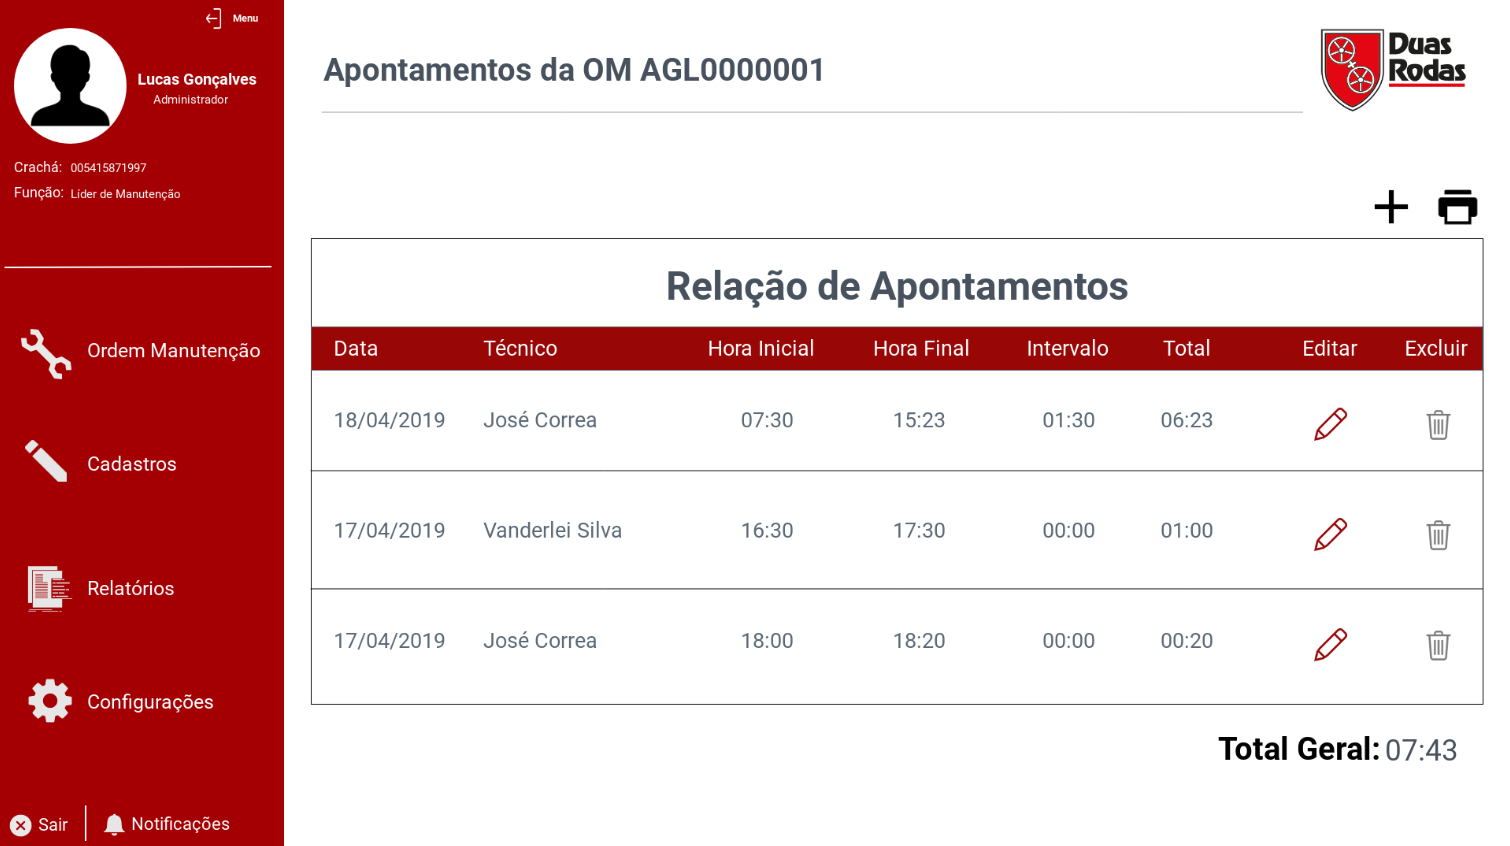
\includegraphics[scale=0.40]{./Figuras/web/om-apontamentos.png}
		\end{center}
		\legend{Fonte: os autores (2020)}
	\end{figure}
	
	Na tela \ref{web_om-apontamentos} será possível visualizar todos os apontamentos que existem em uma ordem, atualizá-las, excluí-las ou adicionar novos apontamentos.
	
	\newpage
	\subsection{Adicionar Apontamentos}
	
	\begin{figure}[htb]
		\caption{\label{web_om-add-apontamento}Adicionar Apontamentos na Ordem de Manutenção}
		\begin{center}
			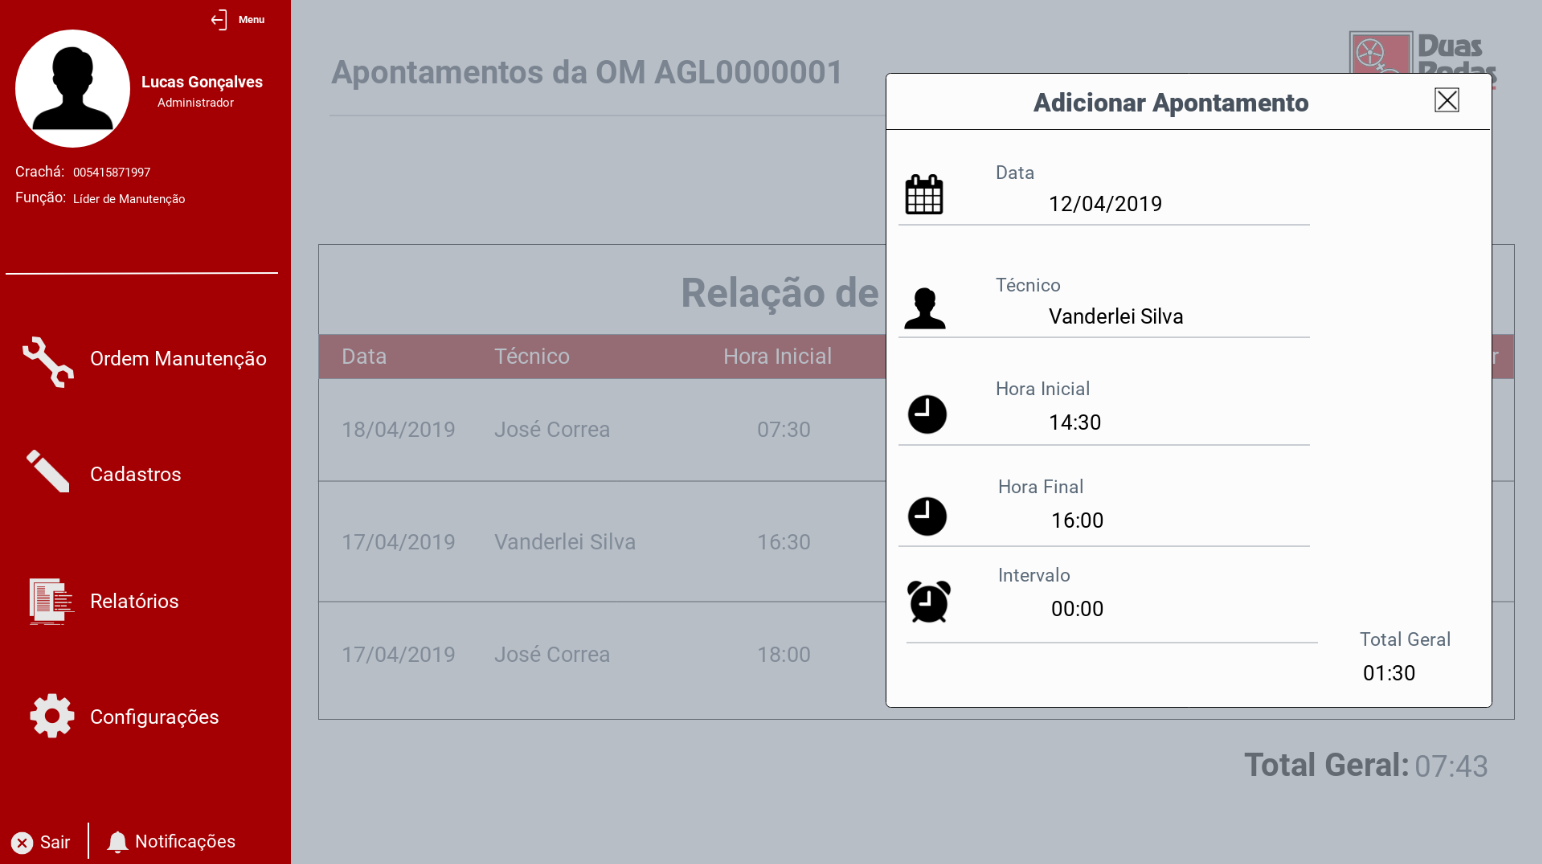
\includegraphics[scale=0.40]{./Figuras/web/om-add-apontamento.png}
		\end{center}
		\legend{Fonte: os autores (2020)}
	\end{figure}
	
	Na tela \ref{web_om-add-apontamento} será possível adicionar novos apontamentos a ordem de manutenção.
	
	\newpage
	\subsection{Motivo da Exclusão do Apontamento da Ordem de Manutenção}
	
	\begin{figure}[htb]
		\caption{\label{web_om-excluir-apontamento-motivo}Motivo da Exclusão do Apontamento da Ordem de Manutenção}
		\begin{center}
			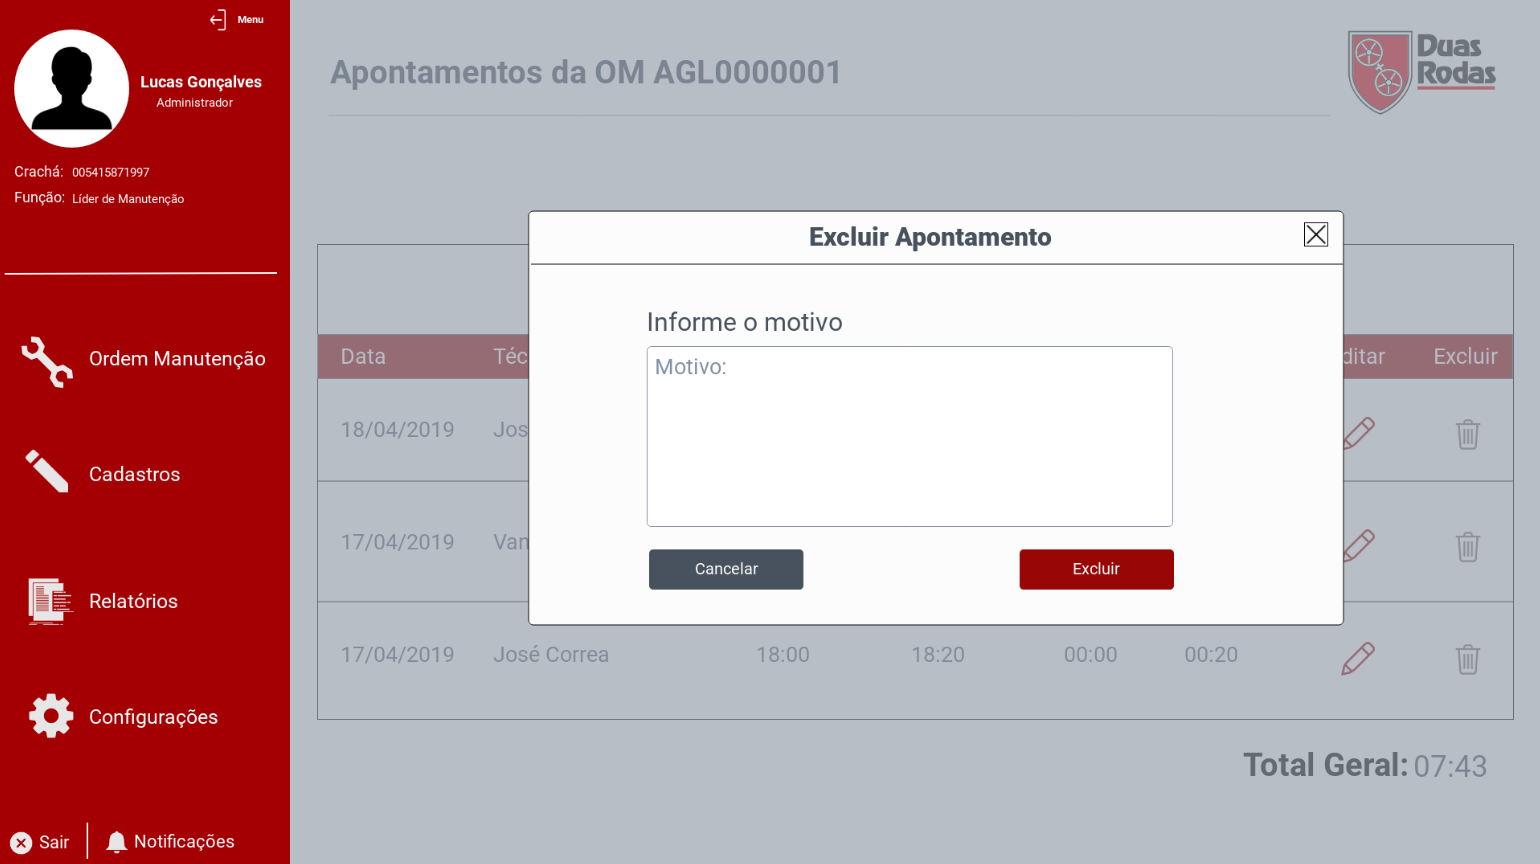
\includegraphics[scale=0.40]{./Figuras/web/om-excluir-apontamento-motivo.png}
		\end{center}
		\legend{Fonte: os autores (2020)}
	\end{figure}
	
	Na tela \ref{web_om-excluir-apontamento-motivo} o operador terá de informar o motivo pela exclusão do apontamento da ordem de manutenção.
	
	\newpage
	\subsection{Assinatura Digital}
	
	\begin{figure}[htb]
		\caption{\label{web_om-assinatura}Assinatura Digital}
		\begin{center}
			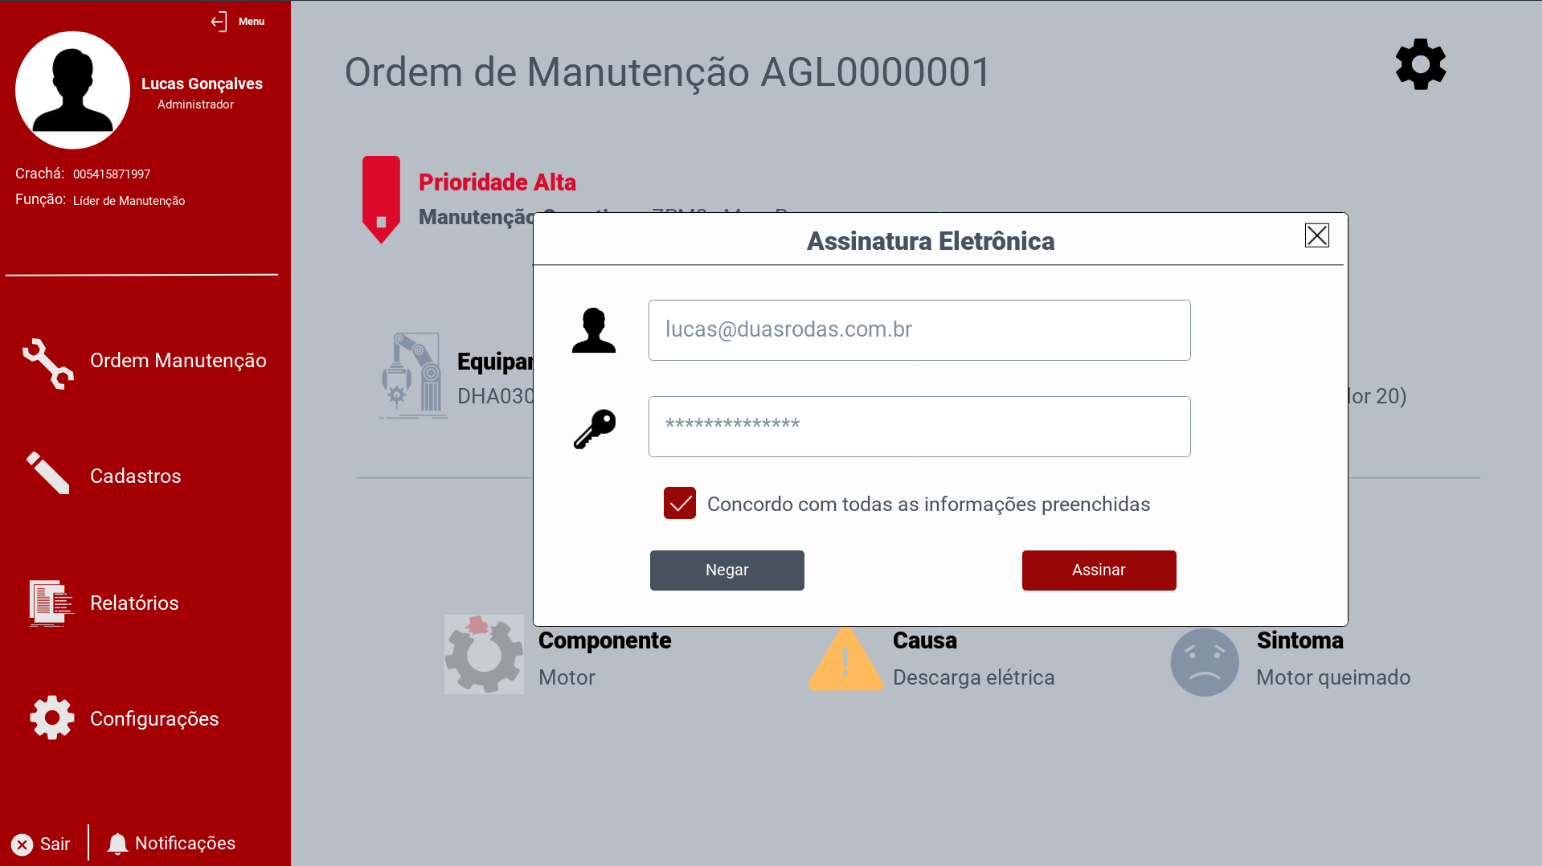
\includegraphics[scale=0.40]{./Figuras/web/om-assinatura.png}
		\end{center}
		\legend{Fonte: os autores (2020)}
	\end{figure}
	
	Na tela \ref{web_om-assinatura} será possível assinar a ordem digitalmente. Para tanto, será cobrado as credenciais do operador.
	
	\newpage
	\section{Aplicação Mobile}
	A aplicação Mobile é um ponto estratégico do produto, pois sua mobilidade permite com que os técnicos possam atuar na manutenção e realizar anotações e apontamentos no sistema através de um smartphone ou tablet.
	
	\subsection{Login}
	
	\begin{figure}[htb]
		\caption{\label{mobile_login}Login}
		\begin{center}
			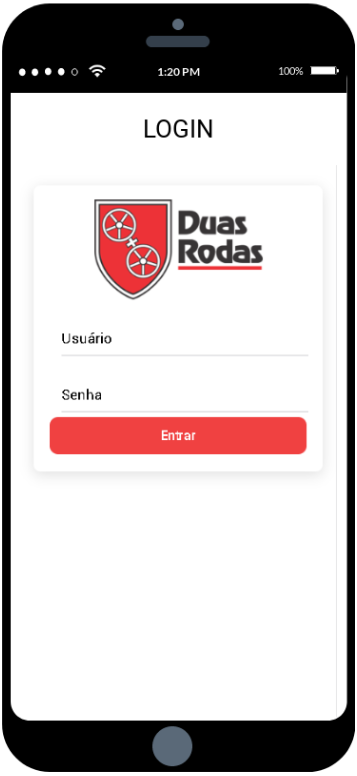
\includegraphics[scale=0.80]{./Figuras/mobile/login.png}
		\end{center}
		\legend{Fonte: os autores (2020)}
	\end{figure}
	
	A tela \ref{mobile_login} será a página responsável por autenticar o usuário e garantir a segurança do sistema.
	
	\newpage
	\subsection{Menu}
	
	\begin{figure}[htb]
		\caption{\label{mobile_menu}Menu}
		\begin{center}
			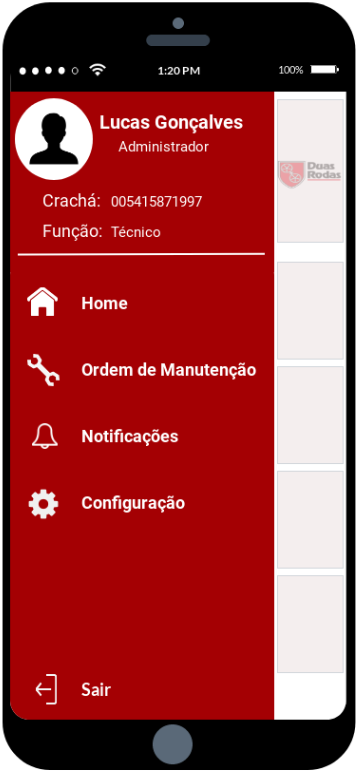
\includegraphics[scale=0.80]{./Figuras/mobile/menu.png}
		\end{center}
		\legend{Fonte: os autores (2020)}
	\end{figure}
	
	A figura \ref{mobile_menu} demonstra o menu lateral do aplicativo, identificando o usuário autenticado e um menu de acesso rápido às principais telas do sistema.
	
	\newpage
	\subsection{Monitor}
	
	\begin{figure}[htb]
		\caption{\label{mobile_monitor}Monitor}
		\begin{center}
			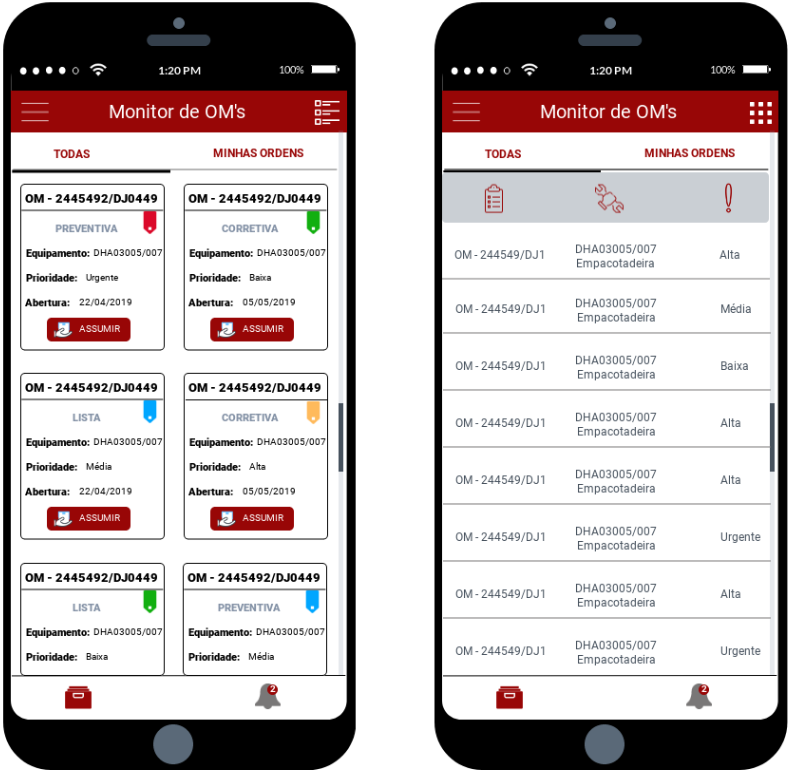
\includegraphics[scale=0.75]{./Figuras/mobile/monitor.png}
		\end{center}
		\legend{Fonte: os autores (2020)}
	\end{figure}
	
	Na figura \ref{mobile_monitor} é possível verificar o monitor do manutentor. Nesse monitor, o manutentor consegue rapidamente visualizar as OMs pendentes e seus respectivos status através das bandeiras indicadas no card. As  vermelhas indicam que a OM tem uma prioridade emergente, as amarelas têm prioridade alta, as azuis têm prioridade média e as verdes possuem uma prioridade baixa.
	
	\newpage
	\subsection{Central de Notificações}
	
	\begin{figure}[htb]
		\caption{\label{mobile_notificacao}Notificações}
		\begin{center}
			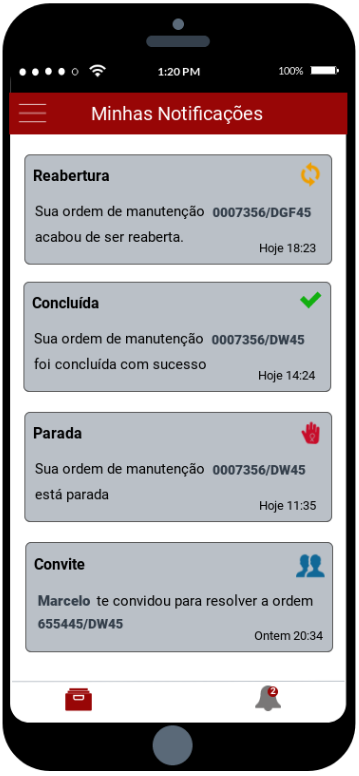
\includegraphics[scale=0.80]{./Figuras/mobile/notificacao.png}
		\end{center}
		\legend{Fonte: os autores (2020)}
	\end{figure}
	
	Na tela \ref{mobile_notificacao} é possível verificar notificações do usuário autenticado no sistema.
	
	\newpage
	\subsection{Ordem de Manutenção}
	
	\begin{figure}[htb]
		\caption{\label{mobile_om}Ordem de Manutenção}
		\begin{center}
			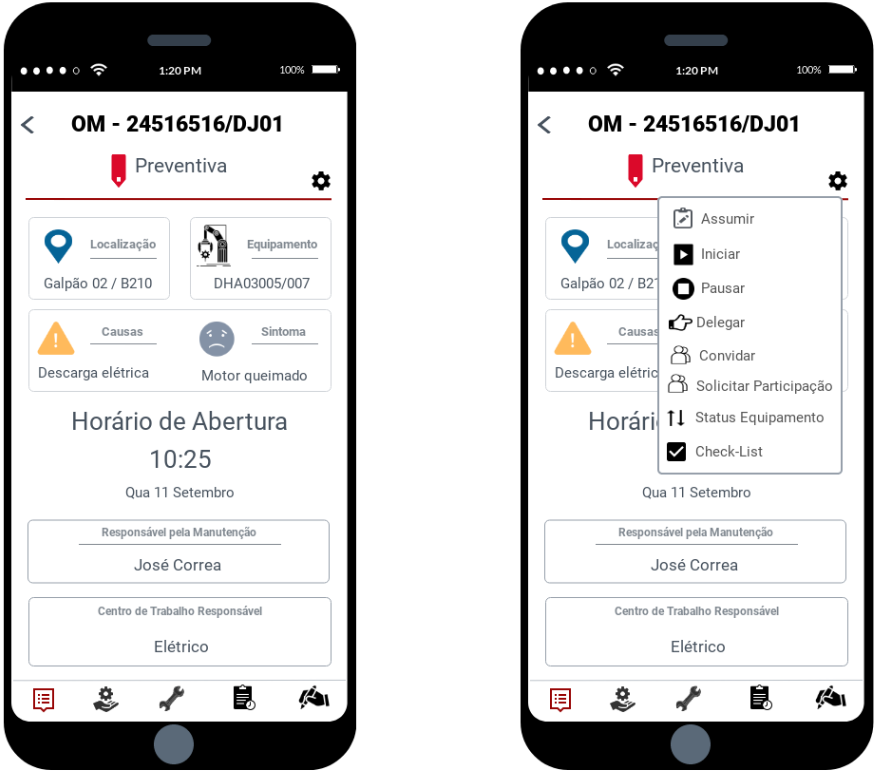
\includegraphics[scale=0.70]{./Figuras/mobile/om.png}
		\end{center}
		\legend{Fonte: os autores (2020)}
	\end{figure}
	
	Na tela \ref{mobile_om} será possível acompanhar o andamento de uma ordem de manutenção preventiva e corretiva, ver informações referente à ordem e executar ações nela, como alterar status, adicionar operações e realizar assinaturas.
	
	\newpage
	\subsection{Ordem de Manutenção: Lista}
	
	\begin{figure}[htb]
		\caption{\label{mobile_lista}Ordem de Manutenção: Lista}
		\begin{center}
			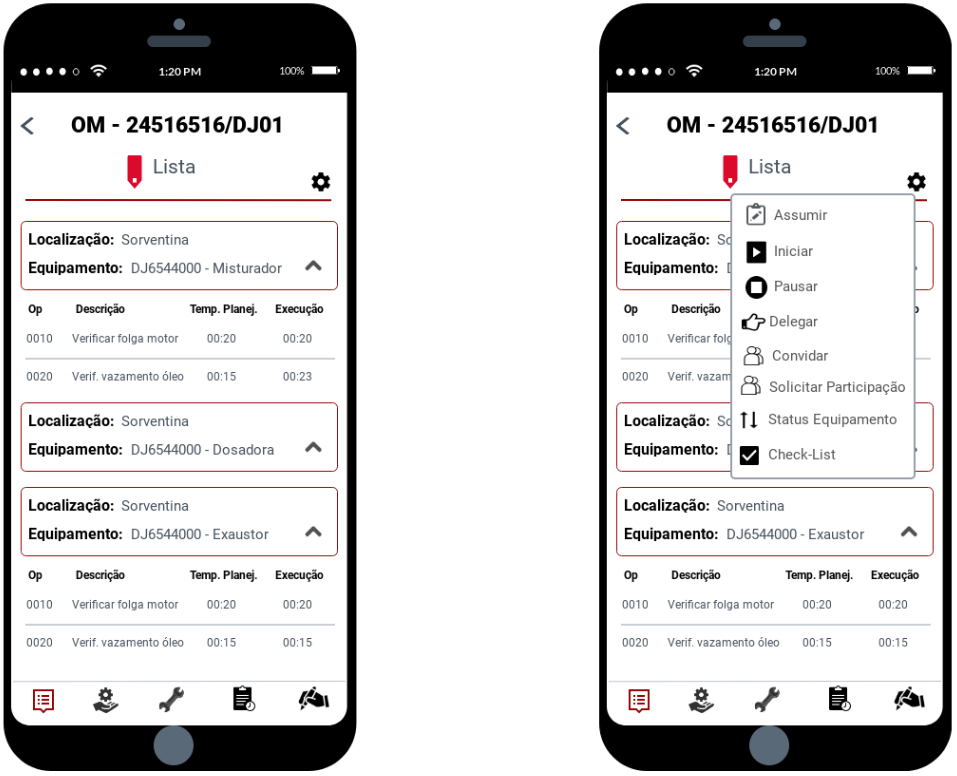
\includegraphics[scale=0.65]{./Figuras/mobile/lista.png}
		\end{center}
		\legend{Fonte: os autores (2020)}
	\end{figure}
	
	Na tela \ref{mobile_lista} será possível acompanhar o andamento de uma ordem de manutenção de lista, ver informações referente à ordem e executar ações nela, como alterar status, adicionar operações e realizar assinaturas.
	
	\newpage
	\subsection{Ordem de Manutenção: Rota}
	
	\begin{figure}[htb]
		\caption{\label{mobile_rota}Ordem de Manutenção: Rota}
		\begin{center}
			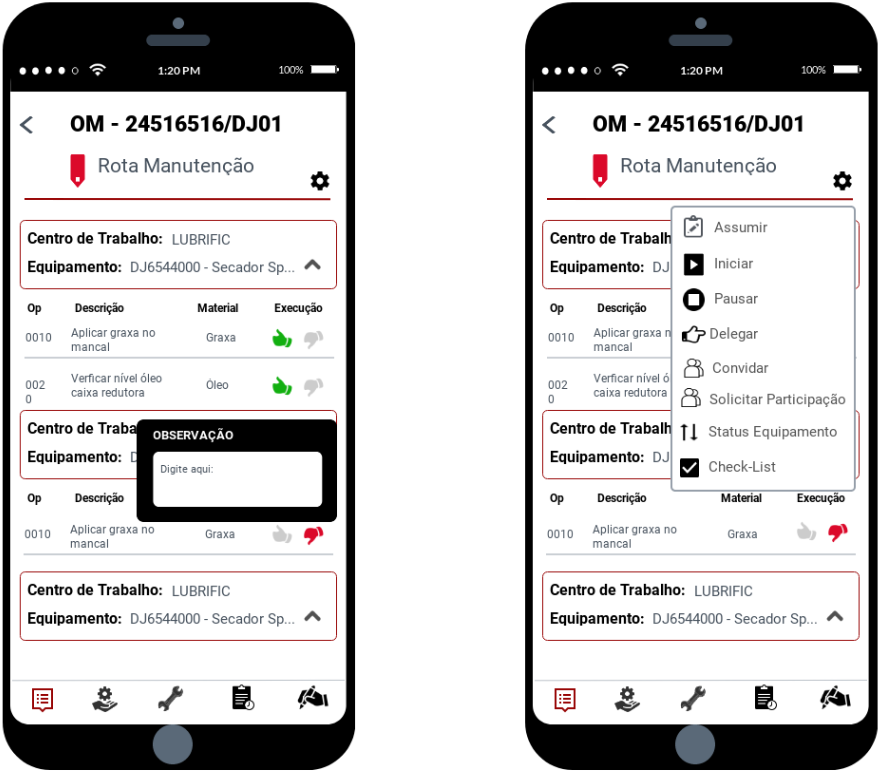
\includegraphics[scale=0.70]{./Figuras/mobile/rota.png}
		\end{center}
		\legend{Fonte: os autores (2020)}
	\end{figure}
	
	Na tela \ref{mobile_rota} será possível acompanhar o andamento de uma ordem de manutenção de rota, ver informações referente à ordem e executar ações nela, como alterar status, adicionar operações e realizar assinaturas.
	
	\newpage
	\subsection{Checklist de Segurança}
	
	\begin{figure}[htb]
		\caption{\label{mobile_checklist}Checklist de Segurança}
		\begin{center}
			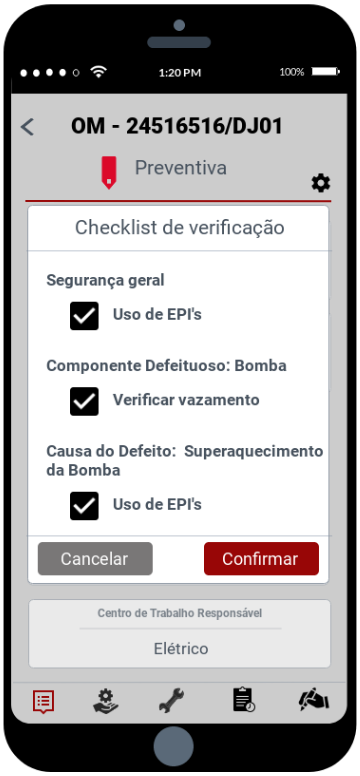
\includegraphics[scale=0.80]{./Figuras/mobile/checklist.png}
		\end{center}
		\legend{Fonte: os autores (2020)}
	\end{figure}
	
	Na tela \ref{mobile_checklist} o manutentor irá marcar a lista de segurança antes de iniciar a ordem de manutenção.
	
	\newpage
	\subsection{Problemas}
	
	\begin{figure}[htb]
		\caption{\label{mobile_problema}Problemas}
		\begin{center}
			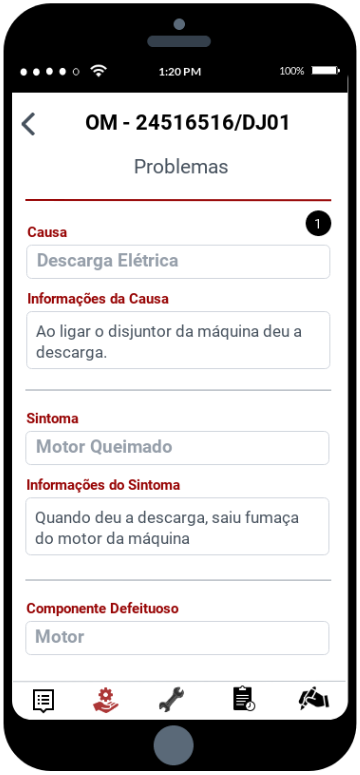
\includegraphics[scale=0.80]{./Figuras/mobile/problemas.png}
		\end{center}
		\legend{Fonte: os autores (2020)}
	\end{figure}
	
	Na tela \ref{mobile_problema} o manutentor irá verificar com maiores detalhes os problemas identificados no equipamento.
	
	\newpage
	\subsection{Componentes}
	
	\begin{figure}[htb]
		\caption{\label{mobile_componentes}Componentes da Ordem de Manutenção}
		\begin{center}
			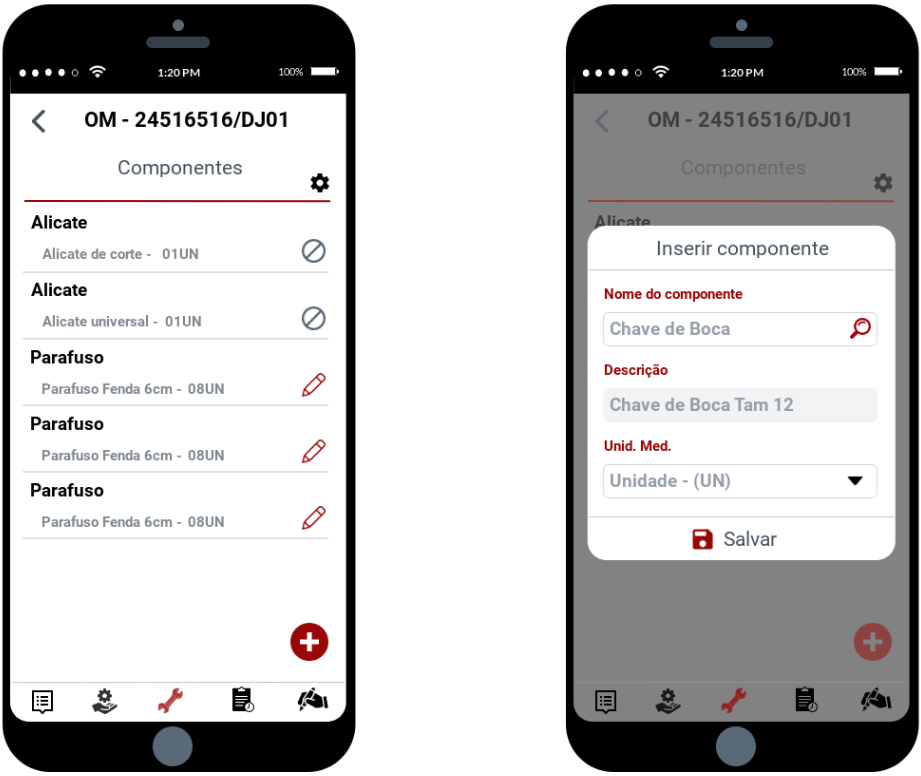
\includegraphics[scale=0.70]{./Figuras/mobile/componentes.png}
		\end{center}
		\legend{Fonte: os autores (2020)}
	\end{figure}
	
	Na tela \ref{mobile_componentes} é possível verificar todos os componentes utilizados na operação da ordem de manutenção.
	
	\newpage
	\subsection{Operações}
	
	\begin{figure}[htb]
		\caption{\label{mobile_operacao}Operações da Ordem de Manutenção}
		\begin{center}
			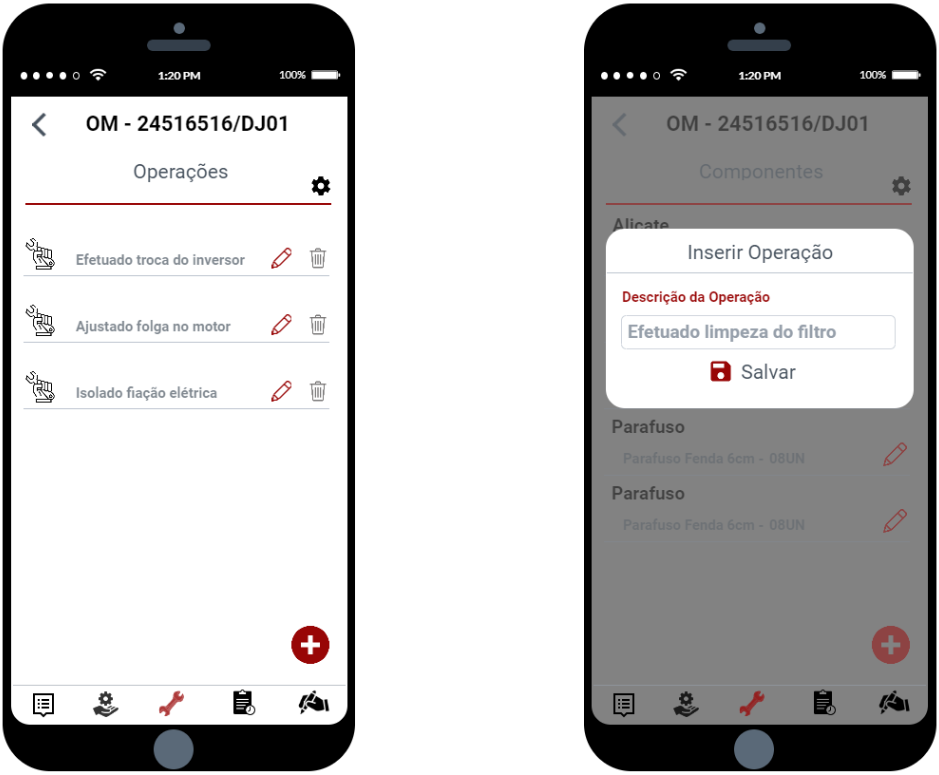
\includegraphics[scale=0.70]{./Figuras/mobile/operacao.png}
		\end{center}
		\legend{Fonte: os autores (2020)}
	\end{figure}
	
	Na tela \ref{mobile_operacao} é possível verificar todas as operações pré cadastradas para a OM e cadastrar novas operações conforme necessidade para o andamento da OM.
	
	\newpage
	\subsection{Apontamentos}
	
	\begin{figure}[htb]
		\caption{\label{mobile_apontamentos}Apontamentos da Ordem de Manutenção}
		\begin{center}
			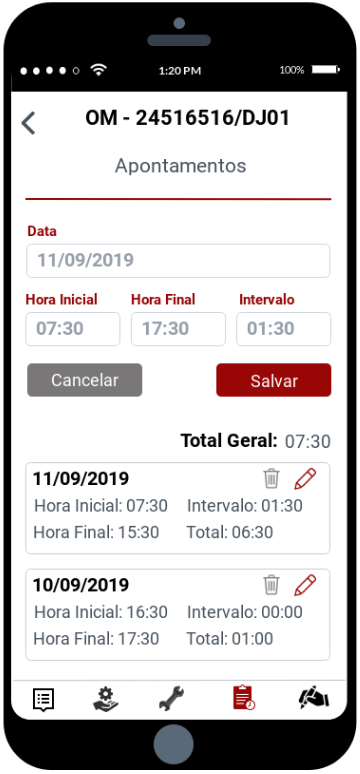
\includegraphics[scale=0.80]{./Figuras/mobile/apontamentos.png}
		\end{center}
		\legend{Fonte: os autores (2020)}
	\end{figure}
	
	Na tela \ref{mobile_apontamentos} é possível realizar os apontamentos das horas trabalhadas na execução da ordem de manutenção.
	
	\newpage
	\subsection{Assinatura Digital}
	
	\begin{figure}[htb]
		\caption{\label{mobile_assinaturas}Assinatura Digital}
		\begin{center}
			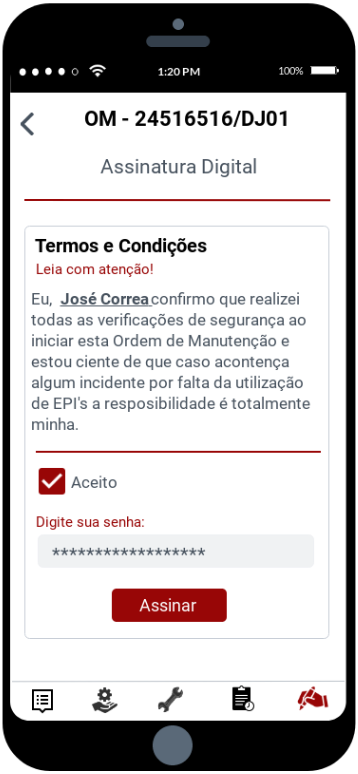
\includegraphics[scale=0.80]{./Figuras/mobile/assinaturas.png}
		\end{center}
		\legend{Fonte: os autores (2020)}
	\end{figure}
	
	Na tela \ref{mobile_assinaturas} é possível verificar e realizar as assinaturas.